\chapter{Irreducibility and factorization in integral domains}
\label{chap:irred}

We move our attention back to \emph{rings} and analyze several useful classes
of integral domains.  One guiding theme in this chapter is the issue of
\emph{factorization}: we will address the problem of existence and uniqueness
of factorizations of elements in a ring, abstracting good factorization
properties of rings such as $\mathbb{Z}$ or $k[x]$ (for $k$ a field) to whole
classes of integral domains.  The reader may want to associate the following
picture with the first part of this chapter:

\begin{center}
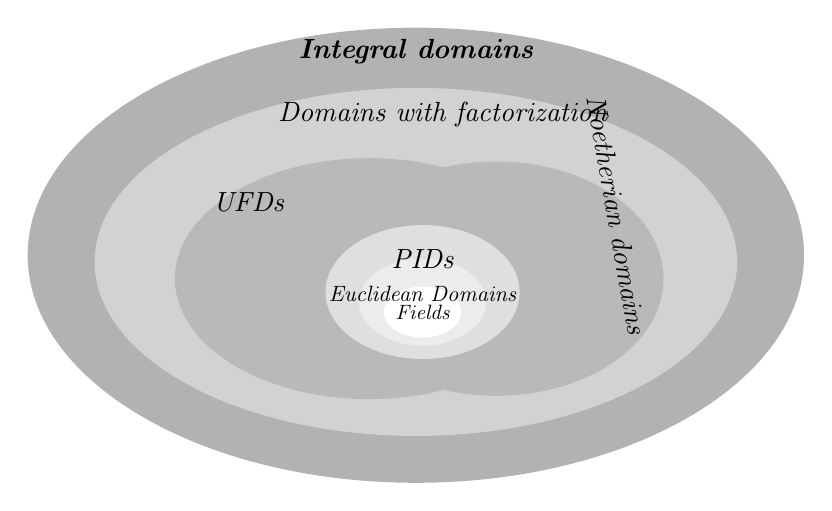
\begin{tikzpicture}[scale=0.85]
  \fill[gray!60] (0,0) ellipse (5.8cm and 3.4cm);
  \fill[gray!35] (0,-0.1) ellipse (4.8cm and 2.6cm);
  \fill[gray!55] (-0.7,-0.35) ellipse (2.9cm and 1.8cm);
  \fill[gray!55] (1.2,-0.35) ellipse (2.5cm and 1.75cm);
  \fill[gray!25] (0.1,-0.55) ellipse (1.45cm and 1.0cm);
  \fill[gray!15] (0.1,-0.7) ellipse (0.95cm and 0.65cm);
  \fill[white] (0.1,-0.85) ellipse (0.58cm and 0.38cm);
  \node[font=\bfseries\itshape] at (0,3.05) {Integral domains};
  \node[font=\itshape] at (0.4,2.1) {Domains with factorization};
  \node[font=\itshape] at (-2.5,0.8) {UFDs};
  \node[font=\itshape, rotate=-80] at (3.0,0.6) {Noetherian domains};
  \node[font=\itshape] at (0.1,-0.05) {PIDs};
  \node[font=\itshape, scale=0.8] at (0.1,-0.58) {Euclidean Domains};
  \node[font=\itshape, scale=0.75] at (0.1,-0.85) {Fields};
\end{tikzpicture}
\end{center}

\emph{Blanket assumption}: all rings considered in this chapter will be
\emph{commutative}\footnote{Also, recall that all our rings have 1; cf.\
Definition~III.1.1.}.  In fact, most of the special classes of rings we will
consider will be \emph{integral domains}, that is, commutative rings with 1
and with no nonzero zero-divisors (cf.\ Definition~III.1.10).

\section{Chain conditions and existence of factorizations}
\label{sec:irred:chain-conditions-and-existence-of-factorizations}


\subsection{Noetherian rings revisited}
\label{subsec:irred:noetherian-rings-revisited}

Let $R$ be a commutative ring. Recall that $R$ is said to be \emph{Noetherian}
if every ideal of $R$ is finitely generated (Definition~III.4.2). In fact,
this is a special case of the corresponding definition for modules: a module
$M$ over a ring $R$ is Noetherian if every submodule of $M$ is finitely
generated (Definition~III.6.6). In~\S{}III.6.4 we have verified that this
condition is preserved through exact sequences: if $M$, $N$, $P$ are
$R$-modules and
\[0 \longrightarrow N \longrightarrow M \longrightarrow P \longrightarrow 0\]
is an exact sequence of $R$-modules, then $M$ is Noetherian if and only if
both $N$ and $P$ are Noetherian (Proposition~III.6.7). An easy and useful
consequence of this fact is that every finitely generated module over a
Noetherian ring is Noetherian (Corollary~III.6.8).

The Noetherian condition may be expressed in alternative ways, and it is
useful to acquire some familiarity with them.
\begin{prop}{}{irred:1.1}
Let $R$ be a commutative ring, and let $M$ be an $R$-module. Then the
following are equivalent:
\begin{enumerate}[label=(\arabic*)]
\item $M$ is Noetherian; that is, every submodule of $M$ is finitely
  generated.
\item Every ascending chain of submodules of $M$ stabilizes; that is, if
  \[N_1 \subseteq N_2 \subseteq N_3 \subseteq \dots\]
  is a chain of submodules of $M$, then $\exists i$ such that
  $N_i = N_{i+1} = N_{i+2} = \dots$
\item Every nonempty family of submodules of $M$ has a maximal element
  w.r.t.\ inclusion.
\end{enumerate}
\end{prop}

The second condition listed here is called the \emph{ascending chain
condition} (a.c.c.) for submodules. For $M = R$, \cref{prop:irred:1.1}
tells us (among other things) that a ring is Noetherian if and only if the
ascending chain condition holds for its ideals.
\begin{proof}
$(1) \implies (2)$: Assume that $M$ is Noetherian, and let
$N_1 \subseteq N_2 \subseteq N_3 \subseteq \dots$ be a chain of submodules
of $M$. Consider the union $N = \bigcup_i N_i$: the reader will verify that
$N$ is a submodule of $M$. Since $M$ is Noetherian, $N$ is finitely
generated, say $N = \langle n_1, \dots, n_r \rangle$. Now $n_k \in N
\implies n_k \in N_i$ for some $i$; by picking the largest such $i$, we
see that $\exists i$ such that all $n_1, \dots, n_r$ are contained in
$N_i$. But then $N \subseteq N_i$, and since $N_i \subseteq N_{i+1}
\subseteq \dots$ are all contained in $N = N_i$, it follows that
$N_i = N_{i+1} = N_{i+2} = \dots$ as needed.

$(2) \implies (3)$: Arguing contrapositively, assume that $M$ admits a
family $\mathscr{F}$ of submodules that does not have a maximal element.
Construct an infinite ascending chain as follows: let $N_1$ be any element
of $\mathscr{F}$; since $N_1$ is not maximal in $\mathscr{F}$, there exists
an element $N_2$ of $\mathscr{F}$ such that $N_1 \subsetneq N_2$; since
$N_2$ is not maximal in $\mathscr{F}$, there exists an element $N_3$ of
$\mathscr{F}$ such that $N_2 \subsetneq N_3$; etc.\ The chain
$N_1 \subsetneq N_2 \subsetneq N_3 \subsetneq \dots$ does not stabilize,
showing that $(2)$ does not hold.

$(3) \implies (1)$: Assume $(3)$ holds, and let $N$ be a submodule of $M$.
Then the family $\mathscr{F}$ of finitely generated submodules of $N$ is
nonempty (as $(0) \in \mathscr{F}$); hence it has a maximal element $N'$.
Say that $N' = \langle n_1, \dots, n_r \rangle$. Now I claim that $N' = N$:
indeed, let $n \in N$; the submodule $\langle n_1, \dots, n_r, n \rangle$
is finitely generated, and therefore it is in $\mathscr{F}$; as it contains
$N'$ and $N'$ is maximal, necessarily $\langle n_1, \dots, n_r, n \rangle
= N'$; in particular $n \in N'$, as needed. This shows that $N = N'$ is
finitely generated, and since $N \subseteq M$ was arbitrary, this implies
that $M$ is Noetherian.
\end{proof}
Noetherian rings are a very useful and flexible class of rings. In~\S{}III.6.5
I mentioned the important fact that every \emph{finite-type algebra} over a
Noetherian ring is Noetherian. `Finite-type (commutative) algebra' is just a
fancy name for a quotient of a polynomial ring (\S{}III.6.5), so this is what
the fact states:

\begin{thm}{}{irred:1.2}
Let $R$ be a Noetherian ring, and let $J$ be an ideal of the polynomial ring
$R[x_1, \dots, x_n]$. Then the ring $R[x_1, \dots, x_n]/J$ is Noetherian.
\end{thm}

Note that finite-type $R$-algebras are (in general) very far from being
finitely generated as modules over $R$ (cf.\ again \S{}III.6.5), so it would
be foolish to expect them to be Noetherian as $R$-modules. The fact that they
turn out to be Noetherian as rings (that is, as modules over themselves)
provides us with a huge class of examples of Noetherian rings, among which are
the rings of (classical) algebraic geometry and number theory. Thus, entire
fields of mathematics are a little more manageable thanks to
\cref{thm:irred:1.2}.

The proof of this deep fact is surprisingly easy. By Exercise~1.1, it suffices
to prove that $R$ Noetherian $\implies$ $R[x_1, \dots, x_n]$ Noetherian; and
an immediate induction reduces the statement to the following particular case,
which carries a distinguished name:
\begin{lem}{Hilbert's basis theorem}{irred:1.3}
$R$ Noetherian $\implies$ $R[x]$ Noetherian.
\end{lem}

\begin{proof}
Assume $R$ is Noetherian, and let $I$ be an ideal of $R[x]$. We have to
prove that $I$ is finitely generated.

Recall that if $f(x) = a_d x^d + a_{d-1} x^{d-1} + \dots + a_0 \in R[x]$
and $a_d \neq 0$, then $a_d$ is called the \emph{leading coefficient} of
$f(x)$. Consider the following subset of $R$:
\[A = \{0\} \cup \{a \in R \mid a \text{ is a leading coefficient of an
  element of } I\}.\]
It is clear that $A$ is an ideal of $R$ (Exercise~1.6); since $R$ is
Noetherian, $A$ is finitely generated. Thus there exist elements
$f_1(x), \dots, f_r(x) \in I$ whose leading coefficients $a_1, \dots, a_r$
generate $A$ as an ideal of $R$.

Now let $d_i$ be the degree of $f_i(x)$, and let $d$ be the maximum among
these degrees. Consider the sub-$R$-module
\[M = \langle 1, x, x^2, \dots, x^{d-1} \rangle \subseteq R[x],\]
that is, the $R$-module consisting of polynomials of degree $< d$. Since
$M$ is finitely generated as a module over $R$, it is Noetherian as an
$R$-module (by Corollary~III.6.8). Therefore, the submodule $M \cap I$ of
$M$ is finitely generated over $R$, say by $g_1(x), \dots, g_s(x) \in I$.

\begin{fact}{Claim~1.4}{irred:claim:1.4}
$I = (f_1(x), \dots, f_r(x), g_1(x), \dots, g_s(x))$.
\end{fact}

This claim implies the statement of the theorem. To prove the claim, we
only need to prove the $\subseteq$ inclusion; to this end, let $\alpha(x)
\in I$ be an arbitrary polynomial in $I$. If $\deg\alpha(x) \geq d$, let
$a$ be the leading coefficient of $\alpha(x)$. Then $a \in A$, so $\exists
b_1, \dots, b_r \in R$ such that $a = b_1 a_1 + \dots + b_r a_r$. Letting
$e = \deg\alpha(x)$, so that $e \geq d_i$ for all $i$, this says that
\[\alpha(x) - b_1 x^{e-d_1} f_1(x) - \dots - b_r x^{e-d_r} f_r(x)\]
has degree $< e$. Iterating this procedure, we obtain a finite list of
polynomials $\beta_1(x), \dots, \beta_r(x) \in R[x]$ such that
\[\alpha(x) - \beta_1(x) f_1(x) - \dots - \beta_r(x) f_r(x)\]
has degree $< d$. But this places this element in $M \cap I$; therefore
$\exists c_1, \dots, c_s \in R$ such that
\[\alpha(x) - \beta_1(x)f_1(x) - \dots - \beta_r(x)f_r(x)
  = c_1 g_1(x) + \dots + c_s g_s(x),\]
and we are done, since this verifies that
\begin{align*}
\alpha(x) &= \beta_1(x)f_1(x) + \dots + \beta_r(x)f_r(x)
             + c_1 g_1(x) + \dots + c_s g_s(x) \\
          &\in (f_1(x), \dots, f_r(x), g_1(x), \dots, g_s(x)),
\end{align*}
completing the proof of \cref{fact:irred:claim:1.4}, hence of
\cref{lem:irred:1.3}, hence of \cref{thm:irred:1.2}.
\end{proof}

\subsection{Prime and irreducible elements}
\label{subsec:irred:prime-and-irreducible-elements}
Let $R$ be a (commutative) ring, and let $a, b \in R$. We say that $a$
\emph{divides} $b$, or that $a$ is a \emph{divisor} of $b$, or that $b$ is a
\emph{multiple} of $a$, if $b \in (a)$, that is,
\[(\exists c \in R),\quad b = ac.\]
We use the notation $a \mid b$.

Two elements $a$, $b$ are \emph{associates} if $(a) = (b)$, that is, if
$a \mid b$ and $b \mid a$.
\begin{lem}{}{irred:1.5}
Let $a$, $b$ be nonzero elements of an integral domain $R$. Then $a$ and
$b$ are associates if and only if $a = ub$, for $u$ a unit in $R$.
\end{lem}

\begin{proof}
Assume $a$ and $b$ are associates. Then $\exists c, d \in R$ such that
$b = ac$, $a = bd$; therefore $a = bd = acd$, i.e., $a(1 - cd) = 0$.
Since cancellation by nonzero elements holds in integral domains, this
implies $cd = 1$. Thus $c$ is a unit, as needed.

The converse is left to the reader.
\end{proof}
Incidentally, here the reader sees why it is convenient to restrict our
attention to integral domains. This argument really shows that if
$(a) = (b) \neq (0)$ in an integral domain, and $b = ca$, then $c$ is
necessarily a unit. Away from the comfortable environment of integral
domains, even such harmless-looking statements may fail: in $\mathbb{Z}/6\mathbb{Z}$
the classes $[2]_6$, $[4]_6$ of 2 and 4 are associates according to our
definition, and $[4]_6 = [2]_6 \cdot [2]_6$, yet $[2]_6$ is not a unit.
However, $[4]_6 = [5]_6 \cdot [2]_6$ and $[5]_6$ is a unit, so this is not
a counterexample to \cref{lem:irred:1.5}. In fact, \cref{lem:irred:1.5}
may fail over rings with `non-harmless' zero-divisors (yes, there is such a
notion).

The notions reviewed above generalize directly the corresponding notions in
$\mathbb{Z}$. We are going to explore analogues of other common notions in
$\mathbb{Z}$, such as `primality' and `irreducibility', in more general
integral domains.
\begin{defn}{}{irred:1.6}
Let $R$ be an integral domain.
\begin{itemize}
\item An element $a \in R$ is \emph{prime} if the ideal $(a)$ is prime;
  that is, $a$ is not a unit and (cf.\ Proposition~III.4.11)
  \[a \mid bc \implies (a \mid b \quad\text{or}\quad a \mid c).\]
\item An element $a \in R$ is \emph{irreducible} if $a$ is not a unit and
  \[a = bc \implies (b \text{ is a unit or } c \text{ is a unit}).\]
\end{itemize}
\end{defn}

Note that $0$ is always reducible (integral domains are nonzero rings!).
For nonzero elements, there are useful alternative ways to think about the
notion of `irreducible': a nonunit $a \neq 0$ is irreducible if and only if
\begin{itemize}
\item $a = bc$ implies that $a$ is an associate of $b$ or of $c$;
\item $a = bc$ implies that $(a) = (b)$ or $(a) = (c)$
  (\cref{lem:irred:1.5});
\item $(a) \subseteq (b) \implies (b) = (a)$ or $(b) = (1)$
  (Exercise~1.12);
\item $(a)$ is maximal among proper principal ideals (rephrasing the
  previous point!).
\end{itemize}

It is important to realize that primality and irreducibility are \emph{not}
equivalent, even for nonzero elements; this is somewhat counterintuitive
since they \emph{are} equivalent in $\mathbb{Z}$, as the reader should
verify\footnote{This fact will be fully explained by the general theory, so
the reader should work this out right away.} (Exercise~1.13). What is true
in general is that prime is stronger than irreducible:

\begin{lem}{}{irred:1.7}
Let $R$ be an integral domain, and let $a \in R$ be a nonzero prime
element. Then $a$ is irreducible.
\end{lem}

\begin{proof}
Since $(a)$ is prime, $(a) \neq (1)$; hence $a$ is not a unit. If
$a = bc$, then $bc = a \in (a)$; therefore $b \in (a)$ or $c \in (a)$
since $(a)$ is prime. Assuming without loss of generality $b \in (a)$, we
have $(b) \subseteq (a)$. On the other hand $a = bc$ implies
$(a) \subseteq (b)$: hence $(a) = (b)$, that is, $a$ and $b$ are
associates, as needed.
\end{proof}

We will soon see under what circumstances the converse statement holds.

\subsection{Factorization into irreducibles; domains with factorizations}
\label{subsec:irred:factorization-into-irreducibles-domains-with-factorizations}

\begin{defn}{}{irred:1.8}
Let $R$ be an integral domain. An element $r \in R$ has a \emph{factorization}
(or \emph{decomposition}) \emph{into irreducibles} if there exist irreducible
elements $q_1, \dots, q_n$ such that $r = q_1 \cdots q_n$.

This factorization is \emph{unique} if the elements $q_i$ are determined by
$r$ up to order and associates, that is, if whenever
$r = q'_1 \cdots q'_m$ is another factorization of $r$ into irreducibles,
then $m = n$ and $q'_i$ is an associate of $q_i$ after (possibly) shuffling
the factors.
\end{defn}

\begin{defn}{}{irred:1.9}
An integral domain $R$ is a \emph{domain with factorizations} (or
`\emph{factorizations exist in} $R$') if every nonzero, nonunit element
$r \in R$ has a factorization into irreducibles.
\end{defn}

\begin{defn}{}{irred:1.10}
An integral domain $R$ is \emph{factorial}, or a \emph{unique factorization
domain} (abbreviated \emph{UFD}), if every nonzero, nonunit element $r \in R$
has a unique factorization into irreducibles.
\end{defn}

The terminology introduced in \cref{defn:irred:1.9} does not appear to be too
standard; by contrast, UFDs are famous.

We will study the unique factorization condition in~\S{}2. For now, it seems
worth spending a little time contemplating the mere existence of
factorizations. Interestingly, this condition is implied by an ascending chain
condition, for a special class of ideals.

\begin{prop}{}{irred:1.11}
Let $R$ be an integral domain, and let $r$ be a nonzero, nonunit element of
$R$. Assume that every ascending chain of principal ideals
\[(r) \subseteq (r_1) \subseteq (r_2) \subseteq (r_3) \subseteq \dots\]
stabilizes. Then $r$ has a factorization into irreducibles.
\end{prop}

\begin{proof}
Assume that $r$ does not have a factorization into irreducible elements. In
particular, $r$ is itself not irreducible; thus $\exists r_1, s_1 \in R$ such
that $r = r_1 s_1$ and $(r) \subsetneq (r_1)$, $(r) \subsetneq (s_1)$. If
both $r_1$, $s_1$ have factorizations into irreducibles, the product of these
factorizations gives a factorization of $r$; thus we may assume that (e.g.)
$r_1$ does not have a factorization into irreducibles. Therefore we have
$(r) \subsetneq (r_1)$ and $r_1$ does not have a factorization; iterating
this argument constructs an infinitely increasing chain
\[(r) \subsetneq (r_1) \subsetneq (r_2) \subsetneq (r_3) \subsetneq \dots,\]
contradicting our hypothesis.
\end{proof}

Thus, factorizations exist in integral domains in which the ascending chain
condition holds for principal ideals. This has the following immediate and
convenient consequence:

\begin{coro}{}{irred:1.12}
Let $R$ be a Noetherian domain. Then factorizations exist in $R$.
\end{coro}

\begin{proof}
By \cref{prop:irred:1.1}, Noetherian domains satisfy the ascending chain
condition for all ideals.
\end{proof}

\cref{coro:irred:1.12} verifies part of the picture presented at the
beginning of the chapter: the class of Noetherian domains is contained in the
class of domains with factorization. This inclusion is proper: for instance,
the standard example of a non-Noetherian ring, $\mathbb{Z}[x_1, x_2, x_3,
\dots]$, (Example~III.6.5) does have factorizations. Indeed, every given
polynomial $f \in \mathbb{Z}[x_1, x_2, \dots]$ involves only finitely many
variables\footnote{Remember that polynomials are finite linear combinations
of monomials; cf.~\S{}III.1.3.}, so it belongs to a subring
$\mathbb{Z}[x_1, \dots, x_n]$ isomorphic to an ordinary polynomial ring over
$\mathbb{Z}$; further, this subring contains every divisor of $f$. It follows
easily (cf.\ Exercise~1.15) that the ascending chain condition for principal
ideals holds in $\mathbb{Z}[x_1, x_2, x_3, \dots]$, because it holds in
$\mathbb{Z}[x_1, \dots, x_n]$ (since this ring is Noetherian, by Hilbert's
basis theorem).

\subsection*{Exercises}

Remember that in this section all rings are taken to be \emph{commutative}.
\begin{exer}{\exerused}{exer:irred:1.1}
Let $R$ be a Noetherian ring, and let $I$ be an ideal of $R$. Prove that
$R/I$ is a Noetherian ring. [\S{}1.1]
\end{exer}

\begin{exer}{}{exer:irred:1.2}
Prove that if $R[x]$ is Noetherian, so is $R$. (This is a `converse' to
Hilbert's basis theorem.)
\end{exer}

\begin{exer}{}{exer:irred:1.3}
Let $k$ be a field, and let $f \in k[x]$, $f \notin k$. For every subring
$R$ of $k[x]$ containing $k$ and $f$, define a homomorphism $\phi : k[t]
\to R$ by extending the identity on $k$ and mapping $t$ to $f$. This makes
every such $R$ a $k[t]$-algebra (Example~III.5.6).
\begin{itemize}
\item Prove that $k[x]$ is finitely generated as a $k[t]$-module.
\item Prove that every subring $R$ as above is finitely generated as a
  $k[t]$-module.
\item Prove that every subring of $k[x]$ containing $k$ is a Noetherian
  ring.
\end{itemize}
\end{exer}

\begin{exer}{}{exer:irred:1.4}
Let $R$ be the ring of real-valued continuous functions on the interval
$[0, 1]$. Prove that $R$ is not Noetherian.
\end{exer}

\begin{exer}{}{exer:irred:1.5}
Determine for which sets $S$ the power set ring $\mathscr{P}(S)$ is
Noetherian. (Cf.\ Exercise~III.3.16.)
\end{exer}
\begin{exer}{\exerused}{exer:irred:1.6}
Let $I$ be an ideal of $R[x]$, and let $A \subseteq R$ be the set defined
in the proof of \cref{thm:irred:1.2}. Prove that $A$ is an ideal of $R$.
[\S{}1.1]
\end{exer}

\begin{exer}{}{exer:irred:1.7}
Prove that if $R$ is a Noetherian ring, then the ring of power series
$R[[x]]$ (cf.~\S{}III.1.3) is also Noetherian. (Hint: The order of a power
series $\sum_{i=0}^{\infty} a_i x^i$ is the smallest $i$ for which $a_i
\neq 0$; the dominant coefficient is then $a_i$. Let $A_i \subseteq R$ be
the set of dominant coefficients of series of order $i$ in $I$, together
with $0$. Prove that $A_i$ is an ideal of $R$ and $A_0 \subseteq A_1
\subseteq A_2 \subseteq \dots$. This sequence stabilizes since $R$ is
Noetherian, and each $A_i$ is finitely generated for the same reason. Now
adapt the proof of \cref{lem:irred:1.3}.)
\end{exer}
\begin{exer}{}{exer:irred:1.8}
Prove that every ideal in a Noetherian ring $R$ contains a finite product
of prime ideals. (Hint: Let $\mathscr{F}$ be the family of ideals that do
not contain finite products of prime ideals. If $\mathscr{F}$ is nonempty,
it has a maximal element $M$ since $R$ is Noetherian. Since $M \in
\mathscr{F}$, $M$ is not itself prime, so $\exists a, b \in R$ s.t.\ $a
\notin M$, $b \notin M$, yet $ab \in M$. What's wrong with this?)
\end{exer}
\begin{exer}{$\lnot$}{exer:irred:1.9}
Let $R$ be a commutative ring, and let $I \subseteq R$ be a proper ideal.
The reader will prove in Exercise~3.12 that the set of prime ideals
containing $I$ has minimal elements (the \emph{minimal primes} of $I$).
Prove that if $R$ is Noetherian, then the set of minimal primes of $I$ is
finite. (Hint: Let $\mathscr{F}$ be the family of ideals that do not have
finitely many minimal primes. If $\mathscr{F} \neq \emptyset$, note that
$\mathscr{F}$ must have a maximal element $I$, and $I$ is not prime itself.
Find ideals $J_1$, $J_2$ strictly larger than $I$, such that $J_1 J_2
\subseteq I$, and deduce a contradiction.) [\hyperref[exer:linAlg:4.10]{VI.4.10}]
\end{exer}
\begin{exer}{$\lnot$}{exer:irred:1.10}
By \cref{prop:irred:1.1}, a ring $R$ is Noetherian if and only if it
satisfies the a.c.c.\ for ideals. A ring is \emph{Artinian} if it
satisfies the d.c.c.\ (descending chain condition) for ideals. Prove that
if $R$ is Artinian and $I \subseteq R$ is an ideal, then $R/I$ is Artinian.
Prove that if $R$ is an Artinian integral domain, then it is a field.
(Hint: Let $r \in R$, $r \neq 0$. The ideals $(r^n)$ form a descending
sequence; hence $(r^n) = (r^{n+1})$ for some $n$. Therefore\dots) Prove
that Artinian rings have Krull dimension $0$ (that is, prime ideals are
maximal in Artinian rings\footnote{One can prove that Artinian rings are
necessarily Noetherian; in fact, a ring is Artinian if and only if it is
Noetherian and has Krull dimension $0$. Thus, the d.c.c.\ implies the
a.c.c., while the a.c.c.\ implies the d.c.c.\ if and only if all prime
ideals are maximal.}). [\hyperref[exer:irred:2.11]{2.11}]
\end{exer}

\begin{exer}{}{exer:irred:1.11}
Prove that the `associate' relation is an equivalence relation.
\end{exer}

\begin{exer}{\exerused}{exer:irred:1.12}
Let $R$ be an integral domain. Prove that a nonzero $a \in R$ is
irreducible if and only if $(a)$ is maximal among proper principal ideals
of $R$. [\S{}1.2, \S{}2.3]
\end{exer}

\begin{exer}{\exerused}{exer:irred:1.13}
Prove that, for nonzero elements, prime $\iff$ irreducible in $\mathbb{Z}$.
[\S{}1.2, \S{}2.3]
\end{exer}

\begin{exer}{}{exer:irred:1.14}
For $a$, $b$ in a commutative ring $R$, prove that the class of $a$ in
$R/(b)$ is prime if and only if the class of $b$ in $R/(a)$ is prime.
\end{exer}

\begin{exer}{\exerused}{exer:irred:1.15}
Identify $S = \mathbb{Z}[x_1, \dots, x_n]$ in the natural way with a
subring of the polynomial ring in countably infinitely many variables
$R = \mathbb{Z}[x_1, x_2, x_3, \dots]$. Prove that if $f \in S$ and
$(f) \subseteq (g)$ in $R$, then $g \in S$ as well. Conclude that the
ascending chain condition for principal ideals holds in $R$, and hence $R$
is a domain with factorizations. [\S{}1.3, \S{}4.3]
\end{exer}

\begin{exer}{}{exer:irred:1.16}
Let
\[R = \frac{\mathbb{Z}[x_1, x_2, x_3, \dots]}{(x_1 - x_2^2,\, x_2 -
x_3^2,\, \dots)}.\]
Does the ascending chain condition for principal ideals hold in $R$?
\end{exer}

\begin{exer}{\exerused}{exer:irred:1.17}
Consider the subring of $\mathbb{C}$:
\[\mathbb{Z}[\sqrt{-5}] := \{a + bi\sqrt{5} \mid a, b \in \mathbb{Z}\}.\]
\begin{itemize}
\item Prove that this ring is isomorphic to $\mathbb{Z}[t]/(t^2 + 5)$.
\item Prove that it is a Noetherian integral domain.
\item Define a `norm' $N$ on $\mathbb{Z}[\sqrt{-5}]$ by setting
  $N(a + bi\sqrt{5}) = a^2 + 5b^2$. Prove that $N(zw) = N(z)N(w)$.
  (Cf.\ Exercise~III.4.10.)
\item Prove that the units in $\mathbb{Z}[\sqrt{-5}]$ are $\pm 1$. (Use
  the preceding point.)
\item Prove that $2$, $3$, $1 + i\sqrt{5}$, $1 - i\sqrt{5}$ are all
  irreducible nonassociate elements of $\mathbb{Z}[\sqrt{-5}]$.
\item Prove that no element listed in the preceding point is prime. (Prove
  that the rings obtained by mod-ing out the ideals generated by these
  elements are not integral domains.)
\item Prove that $\mathbb{Z}[\sqrt{-5}]$ is not a UFD.
\end{itemize}
[\S{}2.2, \hyperref[exer:irred:2.18]{2.18},
\hyperref[exer:irred:6.14]{6.14}]
\end{exer}

\section{UFDs, PIDs, Euclidean domains}
\label{sec:irred:ufds-pids-euclidean-domains}


\subsection{Irreducible factors and greatest common divisor}
\label{subsec:irred:irreducible-factors-and-greatest-common-divisor}
% An integral domain

% R is a UFD if factorizations exist in R and are unique in the sense of
% Definition 1.8.
% Thus, in a UFD all elements (other than 0 and the units) determine a multiset
% (a set of elements `with multiplicity'; cf. \S{}I.1.1) of irreducible factors,
% determined
% up to the associate relation. We can also agree that units have no factors; that
% is,
% the corresponding multiset is \emptyset .
% The following trivial remark is at the root of most elementary facts about
% UFDs, such as the characterization of Theorem 2.5:
% Lemma 2.1. Let R be a UFD, and let a, b, c be nonzero elements of R. Then
% \bullet  (a) \subseteq  (b) \iff  the multiset of irreducible factors of b is contained in the
% multiset of irreducible factors of a;
% \bullet  a and b are associates (that is, (a) = (b)) \iff  the two multisets coincide;
% \bullet  the irreducible factors of a product bc are the collection of all irreducible factors
% of b and of c.
% The proof is left to the reader (Exercise 2.1). The advantage of working in
% a UFD resides in the fact that ring-theoretic statements about elements of the
% ring often reduce to straightforward set-theoretic statements about multisets of
% irreducible elements, by means of Lemma 2.1.
% One important instance of this mechanism is the existence of greatest common
% divisors. I have liberally used this notion (at least for integers) in previous
% chapters;
% now we can appreciate it from a more technical perspective.
% Definition 2.2. Let R be an integral domain, and let a, b \in  R. An element d
% \in  R
% is a greatest common divisor (often abbreviated `gcd') of a and b if (a, b)
% \subseteq  (d) and
% (d) is the smallest principal ideal in R with this property.
%  ?
% In other words, d is a gcd of a and b if d | a, d | b, and
% c | a , c | b \implies  c | d.
% This definition is immediately extended to any finite number of elements.
% Note that greatest common divisors are not defined uniquely by this prescrip-
% tion: if d is a greatest common divisor of a and b, so is every associate of d.
% Thus,
% the notation `gcd(a, b)' should only be used for the associate class formed by
% all
% greatest common divisors of a, b. Of course, language is often (harmlessly)
% abused
% on this point. For example, the fact that we can talk about the greatest common
% divisor of two integers is due to the fact that in Z there is a convenient way
% to choose
% a distinguished element in each class of associate integers (that is, the
% nonnegative
% one).
% Also note that greatest common divisors need not exist (cf. Exercise 2.5); but
% they do exist in UFDs:
% Lemma 2.3. Let R be a UFD, and let a, b be nonzero elements of R. Then a, b
% have a greatest common divisor.
% Proof. We can write
% a = uq1 \alpha 1 \dots  qr \alpha r ,
%  b = vq1 \beta 1 \dots  qr \beta r
% where u and v are units, the elements qi are irreducible, qi is not an associate
% of qj
% for i = j, and \alpha i \geq  0, \beta i \geq  0 (so that the multisets of
% irreducible factors of a,
% resp., b, consist of those qi for which \alpha i > 0, resp., \beta i > 0; the
% units u, v are
% included since the irreducible factors are only defined up to the associate
% relation).
% I claim that
% d = q1
%  min(\alpha 1 ,\beta 1
%  )
%  \dots  qr min(\alpha r ,\beta r )
% is a gcd of a and b. Indeed, d is clearly a divisor of a and b; and if c also
% divides
% a and b, then the multiset of factors of c must be contained in both multisets
% of
% factors for a and b (by Lemma 2.1); that is,
% c = wq1 \gamma 1 \dots  qr \gamma r
% with w a unit and \gamma i \leq  \alpha i , \gamma i \leq  \beta  i . This
% implies \gamma i \leq  min(\alpha i , \beta i ), and hence c | d
% (again by Lemma 2.1), as needed.
%  ?
% Of course the argument given in the proof generalizes one of the standard
% ways to compute greatest common divisors in Z: find smallest exponents in prime
% factorizations. But note that this is not the only way to compute the gcd in Z;
% we will come back to this point in a moment. In fact, greatest common divisors
% in Z have properties that should not be expected in a more general domain: for
% example, the result of Exercise II.2.13 does not generalize to arbitrary domains
% (and not even to arbitrary UFDs), as the reader will check in Exercise 2.4.

\subsection{Characterization of UFDs}
\label{subsec:irred:characterization-of-ufds}
% It is easy to construct integral domains where

% unique factorization fails. The diligent reader has already analyzed one example
% (Exercise 1.17); for another, in the domain5
% C[x, y, z, w]
% R =
% (xw - yz)
% the (classes of the) elements x, y, z, w are irreducible and not associates of
% one
% another; since xw - yz = 0 in R, the element r = xw has two distinct
% factorizations
% into irreducibles: r = xw = yz.
% Note that this ring is Noetherian, by Theorem 1.2 (and in particular factor-
% izations do exist in R). Thus, there are Noetherian integral domains that are
% not
% UFDs.
% Also note that this ring provides an example in which the converse to Lemma 1.7
% does not hold: indeed, (the class of) x is irreducible, but the quotient
% '
% C[x, y, z, w]
%  C[x, y, z, w]
%  C[x, y, z, w]
% (x) \sim 
%  =
%  =
% (xw - yz)
%  (x, xw - yz)
%  (x, yz)
% is not an integral domain (because y = 0, z = 0, and yet yz = 0 in this ring);
% that
% is, x is not prime.
% In fact, and maybe a little surprisingly, the issue of unique factorization is
% inextricably linked with the relation between primality and irreducibility.
% Indeed,
% the `converse' to Lemma 1.7 does hold in UFDs:
% Lemma 2.4. Let R be a UFD, and let a be an irreducible element of R. Then a
% is prime.
% Proof. The element a is not a unit, by definition of irreducible. Assume bc \in
% (a):
% thus (bc) \subseteq  (a), and by Lemma 2.1 the irreducible factors of a, that
% is, a itself,
% must be among the factors of b or of c. We have b \in  (a) in the first case and
% c \in  (a)
% in the second. This shows that (a) is a prime ideal, as needed.
%  ?
% In fact, more is true. Provided that the ascending chain condition for principal
% ideals holds, then UFDs are characterized by the equivalence between
% irreducibility
% and primality.
% Theorem 2.5. An integral domain R is a UFD if and only if
% \bullet  the a.c.c. for principal ideals holds in R and
% \bullet  every irreducible element of R is prime.
% Proof. ( \implies  ) Assume that R is a UFD. Lemma 2.4 shows that irreducible
% ele-
% ments of R are prime. To prove that the a.c.c. for principal ideals holds,
% consider
% an ascending chain
% (r1 ) ? (r2 ) ? (r3 ) ? \dots  .
% 5 In algebraic geometry, this is the ring of a `quadric cone in A4'. The vertex
% of this cone (at
% the origin) is a singular point, and this has to do with the fact that R is not
% a UFD.
% By Lemma 2.1, this chain determines a corresponding descending chain of
% multisets
% of irreducible factors. A descending chain of finite multisets clearly
% stabilizes, and it
% follows (by Lemma 2.1 again) that (ri ) = (ri+1 ) = (ri+2 ) = . . . for large
% enough i.
% ( \Leftarrow = ) Now assume that R satisfies the a.c.c. for principal ideals and
% irre-
% ducibles are prime. Proposition 1.11 implies that factorizations exist in R; we
% have
% \setminus  \setminus to verify uniqueness. Let q1 , . . . , qm and q1 , . . . , qn be irreducible elements of R,
% and assume
% q1 \dots  qm = q1 \setminus  \dots  qn \setminus  .
% Then q1 \setminus  \dots  qn \setminus  \in  (q1 ), and (q1 ) is a prime ideal
% (by hypothesis); thus qi \setminus  \in  (q1)
% for some i, which we may assume to be 1 after changing the order of the factors.
% Therefore q1 \setminus  = uq1 for some u \in  R. Since q1 \setminus  is
% irreducible and q1 is not a unit,
% \setminus  \setminus 
% necessarily u is a unit. Thus q1 and q1 are associates. Canceling q1 and
% replacing q2\setminus by uq2, we find
% q2 \dots  qm = q2 \setminus  \dots  qn \setminus  .
% Repeating this process matches all factors one by one. It is clear that m = n,
% because otherwise we will obtain 1 = a product of irreducibles, contradicting
% the
% fact that irreducibles are not units.
%  ?
% Theorem 2.5 is a pleasant statement, but it does not make it particularly easy
% to
% check whether a given ring is in fact a UFD. The situation is not unlike that
% with
% Noetherian rings: the a.c.c. is a sharp equivalent formulation of the Noetherian
% condition, but in practice one relies more often on other tools, such as
% Hilbert's
% basis theorem, in order to establish that a given ring is Noetherian. Does an
% analog
% of Hilbert's basis theorem hold for unique factorization domains?
% Answering this question requires some preparatory work, and we will come back
% to it in \S{}4.

\subsection{\texorpdfstring{PID $\implies$ UFD}{PID implies UFD}}
\label{subsec:irred:pid-implies-ufd}
% There are simple ways to produce examples of UFDs.

% Recall (from \S{}III.4) that a principal ideal domain (abbreviated PID) is an
% integral
% domain in which every ideal is principal. In \S{}III.4 we have observed that
% \bullet  PIDs are Noetherian.
% \bullet  Z and k[x] (where k is a field) are PIDs.
% \bullet  If R is a PID and a, b \in  R, then d is a greatest common divisor for a and b if
% and only if (a, b) = (d). In particular, if d is a greatest common divisor of a
% and b in a PID R, then d is a linear combination of a and b: \exists r, s \in  R
% such
% that d = ra + sb.
% \bullet  If I is a nonzero ideal in a PID, then I is prime if and only if it is maximal.
% We now add one important point to this list:
% Proposition 2.6. If R is a PID, then it is a UFD.
% Proof. Let R be a PID. The a.c.c. (for principal ideals, as all ideals in R are
% prin-
% cipal!) holds in R since PIDs are Noetherian. We verify that irreducible
% elements
% are prime in R, which implies that R is a UFD by Theorem 2.5.
% Let a \in  R be an irreducible element. Ideals generated by irreducible elements
% are maximal among principal ideals (Exercise 1.12), hence (a) is a maximal ideal
% in R as all ideals in R are principal. Since maximal ideals are prime it follows
% that
% (a) is prime, as needed.
%  ?
% In particular, k[x] is a UFD if k is a field, and Z is a UFD---which hopefully
% will not come as a big surprise to our readers6. Note that at this point we have
% recovered the fact stated in Exercise 1.13 in full glory.
% Proposition 2.6 justifies another feature of the picture given at the beginning
% of this chapter: the class of PIDs is contained in the class of UFDs. We will
% soon
% see that the inclusion is proper, that is, that there are UFDs which are not
% PIDs;
% for example, Z[x] is not a PID (Exercise 2.12), yet
% Z[x] is a unique factorization domain
% as we will soon be able to prove (Theorem 4.14). In fact, there are UFDs which
% are not Noetherian, as represented in the picture; however, these examples are
% best
% discussed after more material has been developed (Example 4.18).
% The reader can already get a feel for the gap between UFD and PID, by con-
% templating the fact (recalled above and essentially tautological) that, in a
% PID,
% greatest common divisors of a, b are linear combinations of a and b. This is a
% very strong requirement: for example, it characterizes PIDs among Noetherian do-
% mains, as the reader will check (Exercise 2.7); it does not hold in general UFDs
% (Exercise 2.4).

\subsection{\texorpdfstring{Euclidean domain $\implies$ PID}{Euclidean domain implies PID}}
\label{subsec:irred:euclidean-domain-implies-pid}
% The excellent properties of Z and k[x] (where

% k is a field) make these rings even more special than PIDs: they are Euclidean
% domains.
% Informally, Euclidean domains are rings in which one may perform a `division
% with remainder': this is the case for Z and for k[x], as observed in \S{}III.4.
% The point
% is that in both Z and k[x] one can define a notion of `size' of an element: |n|
% for an
% integer n and deg f (x) for a polynomial f (x). In both cases, one has control
% over
% the size of the `remainder' in a division. The definition of Euclidean domain
% simply
% abstracts this mechanism.
% For the purpose of this discussion7 , a valuation on an integral domain R is any
% function v : R \setminus  {0} \to  Z\geq 0 .
% Definition 2.7. A Euclidean valuation on an integral domain R is a valuation
% satisfying the following property 8 : for all a \in  R and all nonzero b \in  R
% there exist
% q, r \in  R such that
% a = qb + r,
% with either r = 0 or v(r) < v(b). An integral domain R is a Euclidean domain if
% it
% admits a Euclidean valuation.
%  ?
% 6This fact is known as the fundamental theorem of arithmetic.
% 7 Entire libraries have been written on the subject of valuations, studying a
% more precise
% notion than what is needed here.
% 8 It is not uncommon to also require that v(ab) \geq  v(b) for all nonzero a, b
% \in  R; but this is not
% needed in the considerations that follow, and cf. Exercise 2.15.
% We say that q is the quotient of the division and r is the remainder. Division
% with remainder in Z and in k[x] (where k is a field) provide examples, so that Z
% and k[x] are Euclidean domains.
% Proposition 2.8. Let R be a Euclidean domain. Then R is a PID.
% The proof is modeled after the instances encountered for Z (Proposition III.4.4)
% and k[x] (which the reader has hopefully worked out in Exercise III.4.4).
% Proof. Let I be an ideal of R; we have to prove that I is principal. If I = {0},
% there is nothing to show; therefore, assume I = {0}. The valuation maps the
% nonzero elements of I to a subset of Z\geq 0 ; let b \in  I be an element with
% the smallest
% valuation. Then I claim that I = (b); therefore I is principal, as needed. Since
% clearly (b) \subseteq  I, we only need to verify that I \subseteq  (b).
% For this, let a \in  I and apply division with remainder: we have
% a = qb + r
% for some q, r in R, with r = 0 or v(r) < v(b). But
% r = a - qb \in  I :
% by the minimality of v(b) among nonzero elements of I, we cannot have v(r) <
% v(b).
% Therefore r = 0, showing that a = qb \in  (b), as needed.
%  ?
% Proposition 2.8 justifies one more feature of the picture at the beginning of
% the
% chapter: the class of Euclidean domains is contained in the class of principal
% ideal
% domains.
% This inclusion is proper, as suggested in the picture. Producing an explicit
% example of a PID which is not a Euclidean domain is not so easy, but the gap
% between PIDs and Euclidean domains can in fact be described very sharply: PID
% may be characterized as domains satisfying a weaker requirement than `division
% with remainder'.
% More precisely, a `Dedekind-Hasse valuation' is a valuation v such that \forall
% a, b,
% either (a, b) = (b) (that is, b divides a) or there exists r \in  (a, b) such
% that v(r) < v(b).
% This latter condition amounts to requiring that there exist q, s \in  R such
% that
% as = bq + r with v(r) < v(b); hence a Euclidean valuation (for which we may in
% fact
% choose s = 1) is a Dedekind-Hasse valuation. It is not hard to show that an
% integral
% domain is a PID if and only if it admits a Dedekind-Hasse valuation
%  \sqrt 
%  (Exercise 2.21).
% For example, this can be used to show that the ring Z[(1 + -19)/2] is a PID: the
% norm considered in Exercise 2.18 in order to prove that this ring is not a
% Euclidean
% domain turns out to be a Dedekind-Hasse valuation9 . Thus, this ring gives an
% example of a PID that is not a Euclidean domain.
% One excellent feature of Euclidean domains, and the one giving them their
% names, is the presence of an effective algorithm computing greatest common divi-
% sors: the Euclidean algorithm. As Euclidean domains are PIDs, and hence UFDs,
% we know that they do have greatest common divisors. However, the `algorithm'
% 9 This boils down to a case-by-case analysis, which I am happily leaving to my
% most patient
% readers.
% obtained by distilling the proof of Lemma 2.3 is highly impractical: if we had
% to
% factor two integers a, b in order to compute their gcd, this would make it
% essentially
% impossible (with current technologies and factorization algorithms) for integers
% of
% a few hundred digits. The Euclidean algorithm bypasses the necessity of
% factoriza-
% tion: greatest common divisors of thousand-digit integers may be computed in a
% fraction of a second.
% The key lemma on which the algorithm is based is the following trivial general
% fact:
% Lemma 2.9. Let a = bq + r in a ring R. Then (a, b) = (b, r).
% Proof. Indeed, r = a - bq \in  (a, b), proving (b, r) \subseteq  (a, b); and a =
% bq + r \in  (b, r),
% proving (a, b) \subseteq  (b, r).
%  ?
% In particular,
% (\forall c \in  R),
%  (a, b) \subseteq  (c) \iff  (b, r) \subseteq  (c);
% that is, the set of common divisors of a, b and the set of common divisors of b,
% r
% coincide. Therefore,
% Corollary 2.10. Assume a = bq + r. Then a, b have a gcd if and only if b, r have
% a gcd, and in this case gcd(a, b) = gcd(b, r).
% Of course `gcd(a, b) = gcd(b, r)' means that the two classes of associate
% elements
% coincide.
% These considerations hold over any integral domain; assume now that R is a
% Euclidean domain. Then we can use division with remainder to gain some control
% over the remainders r. Given two elements a, b in R, with b = 0, we can apply
% division with remainder repeatedly:
% a = bq1 + r1 ,
% b = r1 q2 + r2 ,
% r1 = r2 q3 + r3 ,
% \cdot \cdot \cdot 
% as long as the remainder ri is nonzero.
% Claim 2.11. This process terminates: that is, rN = 0 for some N .
% Proof. Each line in the table is a division with remainder. If no ri were zero,
% we
% would have an infinite decreasing sequence
% v(b) > v(r1) > v(r2 ) > v(r3) > \dots 
% of nonnegative integers, which is nonsense.
%  ?
% Thus the table of divisions with remainders must be as follows: letting r0 = b,
% a = r0 q1 + r1 ,
% b = r1 q2 + r2 ,
% r1 = r2 q3 + r3 ,
% \cdot \cdot \cdot 
% rN -3 = rN -2 qN -1 + rN -1 ,
% rN -2 = rN -1 qN
% with rN -1 = 0.
% Proposition 2.12. With notation as above, rN -1 is a gcd of a, b.
% Proof. By Corollary 2.10,
% gcd(a, b) = gcd(b, r1 ) = gcd(r1 , r2 ) = \dots  = gcd(rN -2 , rN -1 ).
% But rN -2 = rN -1 qN -1 gives rN -2 \in  (rN -1 ); hence (rN -2 , rN -1 ) = (rN
% -1 ). There-
% fore rN -1 is a gcd for rN -2 and rN -1 , hence for a and b, as needed.
%  ?
% The ring of integers and the polynomial ring over a field are both Euclidean
% domains. Fields are Euclidean domains (as represented in the picture at the be-
% ginning of the chapter), but not for a very interesting reason: the remainder of
% the
% division by a nonzero element in a field is always zero, so every function
% qualifies
% as a `Euclidean valuation' for trivial reasons.
% We will study another interesting Euclidean domain later in this chapter
% (\S{}6.2).

\subsection*{Exercises}

% 2.1. ? Prove Lemma 2.1. [\S{}2.1]
% 2.2. Let R be a UFD, and let a, b, c be elements of R such that a | bc and
% gcd(a, b) =
% 2.3. Let n be a positive integer. Prove that there is a one-to-one
% correspondence
% preserving multiplicities between the irreducible factors of n (as an integer)
% and
% the composition factors of Z/nZ (as a group). (In fact, the Jordan-H\"older
% theorem
% may be used to prove that Z is a UFD.)
% 2.4. ? Consider the elements x, y in Z[x, y]. Prove that 1 is a gcd of x and y,
% and
% yet 1 is not a linear combination of x and y. (Cf. Exercise II.2.13.) [\S{}2.1,
% \S{}2.3]
% 2.5. ? Let R be the subring of Z[t] consisting of polynomials with no term of
% degree 1: a0 + a2 t2 + \dots  + adtd .
% \bullet  Prove that R is indeed a subring of Z[t], and conclude that R is an integral
% domain.
% \bullet  List all common divisors of t5 and t6 in R.
% \bullet  Prove that t5 and t6 have no gcd in R.
% [\S{}2.1]
% 2.6. Let R be a domain with the property that the intersection of any family of
% principal ideals in R is necessarily a principal ideal.
% \bullet  Show that greatest common divisors exist in R.
% \bullet  Show that UFDs satisfy this property.
% 2.7. ? Let R be a Noetherian domain, and assume that for all nonzero a, b in R,
% the greatest common divisors of a and b are linear combinations of a and b.
% Prove
% that R is a PID. [\S{}2.3]
% 2.8. Let R be a UFD, and let I = (0) be an ideal of R. Prove that every
% descending
% chain of principal ideals containing I must stabilize.
% 2.9. \lnot  The height of a prime ideal P in a ring R is (if finite) the maximum
% length h
% of a chain of prime ideals P0 ? P1 ? \dots  ? Ph = P in R. (Thus, the Krull
% dimension
% of R, if finite, is the maximum height of a prime ideal in R.) Prove that if R
% is a
% UFD, then every prime ideal of height 1 in R is principal. [2.10]
% 2.10. \lnot  It is a consequence of a theorem known as Krull's Hauptidealsatz
% that
% every nonzero, nonunit element in a Noetherian domain is contained in a prime
% ideal of height 1. Assuming this, prove a converse to Exercise 2.9, and conclude
% that a Noetherian domain R is a UFD if and only if every prime ideal of height 1
% in R is principal. [4.16]
% 2.11. Let R be a PID, and let I be a nonzero ideal of R. Show that R/I is an
% artinian ring (cf. Exercise 1.10), by proving explicitly that the d.c.c. holds
% in R/I.
% 2.12. ? Prove that if R[x] is a PID, then R is a field. [\S{}2.3, \S{}VI.7.1]
% 2.13. ? For a, b, c positive integers with c > 1, prove that ca - 1 divides cb -
% 1 if
% and only if a | b. Prove that xa - 1 divides xb - 1 in Z[x] if and only if a |
% b. (Hint:
% For the interesting implications, write b = ad + r with 0 \leq  r < a, and take
% `size'
% into account.) [\S{}VII.5.1, VII.5.13]
% 2.14. ? Prove that if k is a field, then k[[x]] is a Euclidean domain. [\S{}4.3]
% 2.15. ? Prove that if R is a Euclidean domain, then R admits a Euclidean valua-
% tion v such that v(ab) \geq  v(b) for all nonzero a, b \in  R. (Hint: Since R is
% a Euclidean
% domain, it admits a valuation v as in Definition 2.7. For a = 0, let v(a) be the
% minimum of all v(ab) as b \in  R, b = 0. To see that R is a Euclidean domain
% with
% respect to v as well, let a, b be nonzero in R, with b ? a; choose q, r so that
% a = bq+r,
% with v(r) minimal; assume that v(r) \geq  v(b), and get a contradiction.)
% [\S{}2.4, 2.16]
% 2.16. Let R be a Euclidean domain with Euclidean valuation v; assume that
% v(ab) \geq  v(b) for all nonzero a, b \in  R (cf. Exercise 2.15). Prove that
% associate
% elements have the same valuation and that units have minimum valuation.
% 2.17. \lnot  Let R be a Euclidean domain that is not a field. Prove that there
% exists a
% nonzero, nonunit element c in R such that \forall a \in  R, \exists q, r \in  R
% with a = qc + r and
% either r = 0 or r a unit. [2.18]
% \sqrt 
% 2.18. ? For an integer d, denote by Q( d) the smallest subfield of C containing
% \sqrt Q and d, with norm N defined as in Exercise III.4.10. See Exercise 1.17 for the
% case d = -5; in this problem, you will take d = -19.
% \sqrt 
%  \sqrt 
% Let \delta  = (1 + i 19)/2, and consider the following subring of Q( -19):
% ?
%  \sqrt 
% 1 + i 19
% Z[\delta ] := a + b
%  | a, b \in  Z .
% \bullet  Prove that the smallest values of N (z) for z = a + b\delta  \in  Z[\delta ] are 0, 1, 4, 5. Prove
% that N (a + b\delta ) \geq  5 if b = 0.
% \bullet  Prove that the units in Z[\delta ] are \pm 1.
% \bullet  If c \in  Z[\delta ] satisfies the condition specified in Exercise 2.17, prove that c must
% divide 2 or 3 in Z[\delta ], and conclude that c = \pm 2 or c = \pm 3.
% \bullet  Now show that ?q \in  Z[\delta ] such that \delta  = qc + r with c = \pm 2, \pm 3 and r = 0, \pm 1.
% \sqrt 
% Conclude that Z[(1 + -19)/2] is not a Euclidean domain. [\S{}2.4, 6.14]
% 2.19. \lnot  A discrete valuation on a field k is a surjective homomorphism of
% abelian
% groups v : (k\ast  , \cdot ) \to  (Z, +) such that v(a + b) \geq  min(v(a),
% v(b)) for all a, b \in  k\ast  such
% that a + b \in  k\ast  .
% \bullet  Prove that the set R := {a \in  k \ast  | v(a) \geq  0} \cup  {0} is a subring of k.
% \bullet  Prove that R is a Euclidean domain.
% Rings arising in this fashion are called discrete valuation rings, abbreviated
% DVR.
% They arise naturally in number theory and algebraic geometry. Note that the
% Krull dimension of a DVR is 1 (Example III.4.14); in algebraic geometry, DVRs
% correspond to particularly nice points on a `curve'.
% \bullet  Prove that the ring of rational numbers a/b with b not divisible by a fixed prime
% integer p is a DVR.
% [2.20, VIII.1.19]
% 2.20. \lnot  As seen in Exercise 2.19, DVRs are Euclidean domains. In
% particular, they
% must be PIDs. Check this directly, as follows. Let R be a DVR, and let t \in  R
% be an
% element such that v(t) = 1. Prove that if I \subseteq  R is any nonzero ideal,
% then I = (tk )
% for some k \geq  1. (The element t is called a `local parameter' of R.) [4.13,
% VII.2.18]
% 2.21. ? Prove that an integral domain is a PID if and only if it admits a
% Dedekind-
% Hasse valuation. (Hint: For the \Leftarrow = implication, adapt the argument in
% Proposi-
% tion 2.8; for \implies  , let v(a) be the size of the multiset of irreducible
% factors of a.)
% [\S{}2.4]
% 2.22. \lnot  Suppose R \subseteq  S is an inclusion of integral domains, and
% assume that R is
% a PID. Let a, b \in  R, and let d \in  R be a gcd for a and b in R. Prove that d
% is also
% a gcd for a and b in S. [5.2]
% 2.23. Compute d = gcd(5504227617645696, 2922476045110123). Further, find a, b
% such that d = 5504227617645696 a + 2922476045110123 b.

\section{Intermezzo: Zorn's lemma}
\label{sec:irred:intermezzo-zorn-s-lemma}


%Prove that there are infinitely many prime integers. (Hint: Assume by}

% contradiction that p1 , . . . , pN is a complete list of all positive prime
% integers. What
% can you say about p 1 \dots  \cdot  \cdot  pN + 1? This argument was already
% known to Euclid,
% more than 2,000 years ago.) [2.25, \S{}5.2, 5.11]

% \lnot  Variation on the theme of Euclid from Exercise 2.24: Let f (x) \in  Z[x] be

% a nonconstant polynomial such that f (0) = 1. Prove that infinitely many primes
% divide the numbers f (n), as n ranges in Z. (If p1, . . . , pN were a complete
% list of
% primes dividing the numbers f (n), what could you say about f (p1 \dots  pN x)?)
% Once you are happy with this, show that the hypothesis f (0) = 1 is unnecessary.
% (If f (0) = a = 0, consider f (p1 \dots  pN ax). Finally, note that there is
% nothing special
% about 0.) [VII.5.18]

\subsection{Set theory, reprise}
\label{subsec:irred:set-theory-reprise}
% We leave ring theory for a moment and take a little

% detour to contemplate an issue from set theory. As remarked at the very outset,
% only naive set theory is used in this book; all set-theoretic operations we have
% used
% so far are nothing more than a formalization of intuitive ideas regarding
% collections
% of objects. However, I will occasionally need to refer to a less `intuitively
% obvious'
% set-theoretic statement: for example, this statement is needed in order to show
% that
% every proper ideal in a ring is contained in a maximal ideal (Proposition 3.5).
% This set-theoretic fact is Zorn's lemma. An order relation on a set Z is a
% relation ? which is reflexive, transitive, and antisymmetric: the first two
% terms are
% familiar to the reader, and the third means that
% (\forall a, b \in  Z),
%  a ? b and b ? a \implies  a = b.
% Typical prototypes are the \leq  relation on Z or the inclusion relation
% \subseteq  among subsets
% of a given set. We use a \prec  b to denote a ? b and b = a.
% A pair (Z, ?), consisting of a set Z and an order relation ? on Z, is called
% a poset, for partially ordered set. The qualifier `partially' is not necessary,
% but
% convenient, as it reminds us that if a, b \in  Z, then it is not necessarily the
% case
% that a ? b or b ? a: for example, \subseteq  does not satisfy this additional
% requirement
% in general (while (Z, \leq ) does). An order is total if it does satisfy this
% additional
% requirement. A totally ordered set is not called a `toset', as would seem
% reasonable,
% but rather a chain.
% An element m of a poset Z is maximal if nothing comes properly `after' it in
% the order:
% (\forall a \in  Z), m ? a \implies  m = a.
% For example, maximal ideals in a ring are maximal elements in the set of proper
% ideals, that is, ideals = (1) (by Proposition III.4.11). An upper bound for a
% subset S
% of a poset Z is an element u \in  Z coming after every element of S:
% (\forall a \in  S),
%  a ? u.
% Notions of `smallest' (or, rather, `least') or `largest' are defined in the
% evident
% way.
% Posets may or may not have maximal elements, upper bounds, etc.: for exam-
% ple, the family of finite subsets of an infinite set does not have maximal
% elements.
% All this terminology comes together in the following statement:
% Lemma 3.1 (Zorn's lemma). Let Z be a nonempty poset. Assume that every chain
% in Z has an upper bound in Z; then there exists a maximal element in Z.
% The status of Zorn's lemma is peculiar: on the one hand, it is complex enough
% that no one I know of finds it `intuitively clear'; on the other hand, it turns
% out to
% be logically equivalent 10 to the axiom of choice, which does look reasonable to
% most
% people, and to the `well-ordering theorem', which I find intuitively
% unreasonable.
% I will not prove all these equivalences (the diligent reader will prove them in
% the
% exercises and should in any case have no trouble locating more detailed proofs);
% but I will attempt to describe the situation in general terms and explain why
% the
% unreasonable statement implies the other two.
% The axiom of choice states that if F is a family of disjoint nonempty subsets of
% a set Z, then we can form a new set by selecting one element x from each X \in
% F .
% This may sound reasonable, but it raises rather subtle points: for example, it
% can
% be shown that this axiom is independent of the other axioms of
% (Zermelo-Fr\"ankel)
% set theory. Also, it has disturbingly counterintuitive consequences, such as the
% Banach-Tarski paradox11 .
% The subtlety of the axiom of choice boils down to the following question: how
% does one choose the element x? This is not controversial if Z (and hence F ) is
% finite, but, not surprisingly, it becomes an issue if Z is infinite.
% A suitable order relation on Z would come in handy here: if ? is an order
% relation on Z such that every nonempty subset of Z has a least element, then we
% could simply let x be the least element of X for each X \in  F . We say that Z
% is well-ordered by ?, or that ? is a well-ordering on Z, if this is the case.
% (The
% abbreviation woset is also used in the literature, but not very often.) For
% example,
% the set Z>0 of positive numbers is well-ordered by \leq ; this fact is called
% the well-
% ordering principle.
% Thus, the statement of the axiom of choice is really `clear' if the set Z is the
% set Z>0 of positive numbers. It may seem somewhat less so for the set Z, since Z
% is not well-ordered by \leq ; however, it takes a moment (Exercise 3.4) to
% construct a
% different relation on Z, making Z a well-ordered set. Thus, the axiom of choice
% is
% also completely transparent for Z = Z or any countable set (like Q) for that
% matter.
% The well-ordering principle is at the basis of proofs by induction: in fact (cf.
% Ex-
% ercise 3.5) it is equivalent to the so-called principle of induction. More is
% true,
% however. If (Z, ?) is any woset, then we can consider the following `principle
% of
% induction' on Z:
% 10 Equivalent in the sense that each can be derived from the other together with
% the other
% axioms of `Zermelo-Fr\"ankel' set theory.
% 11 One can subdivide a solid ball of radius 1 into finitely many pieces, then
% reassemble them
% after rotations and translations in 3-space and obtain two balls of radius 1.
% Let S \subseteq  Z be a subset such that \forall a \in  Z
% ((\forall b \in  Z),
%  b \prec  a \implies  b \in  S) \implies  a \in  S;
% then S = Z.
% That is, Z is the only set S with the property that a \in  S if all b \prec  a
% are in S.
% (Note that the least element a of Z is automatically in S, since the condition
% on
% all b \prec  a is vacuously true in this case.)
% The reader will recognize that for Z = Z>0 with the relation \leq , this is the
% ordinary principle of induction.
% Claim 3.2. Let Z be any woset. Then the principle of induction holds for Z.
% Proof. Let S \subseteq  Z be a subset with the property given above, and assume
% S ? Z.
% Then the complement T of S in Z is nonempty; hence it has a least element a.
% Now if b \prec  a, then necessarily b \in  S (otherwise b \in  T , contradicting
% the fact that a
% is the least element in T ). But the property of S then forces a \in  S,
% contradiction.
% Therefore T is empty; i.e., S = Z.
%  ?
% This is remarkable, since it extends induction to uncountable sets12 , provided
% a well-ordering is available.
% For example, if we had a well-ordering on R, then we could prove a statement
% about all reals `by induction'. Many people find this somewhat counterintuitive,
% and hence so seems the following amazing claim:
% Theorem 3.3 (Well-ordering theorem). Every set admits a well-ordering.
% As argued above, this implies that the axiom of choice holds on every set: if
% you
% accept the well-ordering theorem, the statement of the axiom of choice becomes
% as
% evident for every set as it is for the set of positive integers. The catch is of
% course
% that the axiom of choice is used in the proof of the well-ordering theorem; in
% fact,
% the statements are equivalent.
% In any case, the statement of the well-ordering theorem is easy to absorb (even
% if perhaps less `intuitively clear' than the axiom of choice). The well-ordering
% theorem is equivalent to Zorn's lemma, since they are both equivalent to the
% axiom
% of choice. The good news is that the derivation of Zorn's lemma from the well-
% ordering theorem is reasonably straightforward:
% Well-ordering theorem \implies  Zorn's lemma. Let (Z, \leq ) be a nonempty poset
% such
% that every chain in Z has an upper bound in Z. By the well-ordering theorem,
% there
% is a well-ordering13 ? on Z. Define a function f from Z to the power set of Z as
% 12 Even beyond; in the context of ordinals this induction principle is called
% transfinite induc-
% tion.
% 13 Watch out: we are considering two orderings on Z: \leq  (about which we want
% to say
% something) and ? (about which we know something already).
% follows:
% \{
%  \setminus 
% |
%  |
%  |
%  {a} if ({a} \cup 
%  f (b)) is totally ordered by \leq ;
% f (a) =
%  b\prec a
%  \setminus 
% |
%  |
%  \} \emptyset  if ({a} \cup 
%  f (b)) is not totally ordered by \leq .
% b\prec a
% The fact that Z is well-ordered by ? implies that f is defined for every a \in
% Z.
% Indeed, let T be the set of elements of Z for which f is not defined; if T =
% \emptyset ,
% T has a least element a w.r.t. ?; but then f (b) is defined for all b \prec  a,
% and the
% prescription given for f (a) defines f at a, a contradiction.
% ?
% Let S = a\in Z f (a). It is clear that S is totally ordered by \leq : if a, b
% \in  S, and
% (say) b \prec  a, then both a and b belong to
% \setminus 
% {a} \cup 
%  f (b),
% b\prec a
% which is totally ordered by \leq  by construction.
% I claim that S is a maximal totally ordered subset14 of Z:
% Claim 3.4. If S \subseteq  S \setminus  \subseteq  Z and S \setminus  is totally
% ordered by \leq , then S = S \setminus  .
% Indeed, let T be the complement of S in S \setminus  . If T is nonempty, let a
% \in  T and
% observe that
%  \setminus 
% {a} \cup 
%  f (b)
% b\prec a
% is totally ordered by \leq , since it is a subset of {a} \cup  S \subseteq  S
% \setminus  . But then f (a) = {a},
% that is, a \in  S, a contradiction.
% Since S is a chain, by the hypothesis of Zorn's lemma S has an upper bound,
% m. It is now clear that m must be maximal in Z w.r.t. \leq , verifying the
% statement
% of Zorn's lemma. Indeed, if m\setminus  \geq  m, then S \cup  {m\setminus  } is
% totally ordered; hence
% S = S \cup  {m\setminus  } by the claim. This means m\setminus  \in  S, and
% hence m\setminus  = m since m is an
% upper bound for S.
%  ?
% Zorn's lemma is the key to several basic results in algebra, the first of which
% we
% are about to encounter; the reader will sample a few more results in the
% exercises.
% The reader will also encounter equally basic applications of Zorn's lemma (or of
% other manifestations of the axiom of choice) in other fields: for example
% Tychonoff's
% theorem in topology and the Hahn-Banach theorem in functional analysis.

\subsection{Application: Existence of maximal ideals}
\label{subsec:irred:application-existence-of-maximal-ideals}
% Recall (\S{}III.4.3) that an

% ideal m of a ring R is maximal if and only if R/m is a field, if and only if no
% other ideal stands between m and R = (1), that is, if and only if m is maximal
% with
% respect to inclusion, in the family of proper ideals of R. It is not obvious
% from this
% definition that maximal ideals exist, but they do:
% Proposition 3.5. Let I = (1) be a proper ideal of a commutative ring R. Then
% there exists a maximal ideal m of R containing I.
% 14 The existence of maximal totally ordered subsets is known as the Hausdorff
% maximal prin-
% ciple; it is also equivalent to the axiom of choice.

\subsection*{Exercises}

% This is immediate if R is Noetherian, by applying condition (3) from Propo-
% sition 1.1 to the family of proper ideals of R containing I. The argument for
% arbitrary rings is a classic application of Zorn's lemma. In fact, this is the
% first
% application given by M. Zorn in his 1935 article introducing a `maximum
% principle'
% (now known as Zorn's lemma). The result had earlier been proven by Krull, using
% the well-ordering theorem.
% Proof. The set I of proper ideals of R containing I is ordered by inclusion.
% Then
% let C be a chain of proper ideals, and consider
% \setminus 
% U :=
%  J.
% J\in C
% I claim that U is a proper ideal containing I; hence it is an upper bound for C
% in I . This proves that every chain in I has an upper bound, and it follows that
% I has maximal elements, by Zorn's lemma.
% To verify my claim, it is clear that U contains I and that it is an ideal (for
% example, if a, b \in  U , then \exists J \in  C such that a, b \in  J; hence a
% \pm  b \in  J, and therefore
% a \pm  b \in  U ). We have to check that U is proper. But if U = (1), then 1 \in
% J for some
% J \in  I , contradicting the fact that I consists of proper ideals.
%  ?
% Note that this argument relies crucially on the fact that R has a multiplicative
% unit 1, and indeed the stated fact is not true in general for rings without 1
% (Exer-
% cise 3.9). Also, the use of Zorn's lemma is not just a convenient trick; the
% statement
% is known to be equivalent to the axiom of choice, by work of W. Hodges.
% 3.1. Prove that every well-ordering is total.
% 3.2. Prove that a totally ordered set (Z, ?) is a woset if and only if every
% descending
% chain
% z1 ! z2 ! z3 ! \dots 
% in Z stabilizes.
% 3.3. Prove that the axiom of choice is equivalent to the statement that a set-
% function is surjective if and only if it has a right-inverse (cf. Exercise
% I.2.2).
% 3.4. ? Construct explicitly a well-ordering on Z. Explain why you know that Q
% can be well-ordered, even without performing an explicit construction. [\S{}3.1]
% 3.5. ? Prove that the (ordinary) principle of induction is equivalent to the
% state-
% ment that \leq  is a well-ordering on Z>0. (To prove by induction that (Z>0,
% \leq )
% is well-ordered, assume it is known that 1 is the least element of Z>0 and that
% \forall n \in  Z >0 there are no integers between n and n + 1.) [\S{}3.1]
% 3.6. In this exercise assume the truth of Zorn's lemma and the conventional set-
% theoretic constructions; you will be proving the well-ordering theorem.
% Let Z be a nonempty set, and let Z be the set of pairs (S, \leq ) consisting of
% a
% subset S of Z and of a well-ordering \leq  on S. Note that Z is not empty
% (singletons
% can be well-ordered). Define a relation ? on Z by prescribing
% (S, \leq ) ? (T, \leq \setminus  )
% if and only if S \subseteq  T , \leq  is the restriction of \leq \setminus  to
% S, and every element of S precedes
% every element of T \setminus  S w.r.t. \leq \setminus  .
% \bullet  Prove that ? is an order relation in Z .
% \bullet  Prove that every chain in Z has an upper bound in Z .
% \bullet  Use Zorn's lemma to obtain a maximal element (M, \leq ) in Z . Prove that
% M = Z.
% Thus every set admits a well-ordering, as stated in Theorem 3.3.
% 3.7. In this exercise assume the truth of the axiom of choice and the
% conventional
% set-theoretic constructions; you will be proving the well-ordering theorem15 .
% Let Z be a nonempty set. Use the axiom of choice to choose an element
% \gamma (S) \in  S for each proper subset S ? Z. Call a pair (S, \leq ) a \gamma -woset if S \subseteq  Z, \leq 
% is a well-ordering on S, and for every a \in  S, a = \gamma ({b \in  S, b < a}).
% \bullet  Show how to begin constructing a \gamma -woset, and show that all \gamma -wosets must
% begin in the same way.
% Define an ordering on \gamma -wosets by prescribing that (U, \leq \setminus
% \setminus  ) ? (T, \leq \setminus  ) if and only if
% U \subseteq  T and \leq \setminus \setminus  is the restriction of \leq
% \setminus  .
% \bullet  Prove that if (U, \leq \setminus \setminus  ) \prec  (T, \leq \setminus ), then \gamma (U ) \in  T .
% \bullet  For two \gamma -wosets (S, \leq ) and (T, \leq \setminus  ), prove that there is a maximal \gamma -woset
% (U, \leq \setminus \setminus  ) preceding both w.r.t. ?. (Note: There is no need
% to use Zorn's lemma!)
% \bullet  Prove that the maximal \gamma -woset found in the previous point in fact equals
% (S, \leq ) or (T, \leq \setminus ). Thus, ? is a total ordering.
% \bullet  Prove that there is a maximal \gamma -woset (M, \leq ) w.r.t. ?. (Again, Zorn's lemma
% need not and should not be invoked.)
% \bullet  Prove that M = Z.
% Thus every set admits a well-ordering, as stated in Theorem 3.3.
% 3.8. Prove that every nontrivial finitely generated group has a maximal proper
% subgroup. Prove that (Q, +) has no maximal proper subgroup.
% 3.9. ? Consider the rng (= ring without 1; cf. \S{}III.1.1) consisting of the
% abelian
% group (Q, +) endowed with the trivial multiplication qr = 0 for all q, r \in  Q.
% Prove
% that this rng has no maximal ideals. [\S{}3.2]
% 3.10. \lnot  As shown in Exercise III.4.17, every maximal ideal in the ring of
% continuous
% real-valued functions on a compact topological space K consists of the functions
% vanishing at a point of K.
% 15I learned this proof from notes of Dan Grayson.

\section{Unique factorization in polynomial rings}
\label{sec:irred:unique-factorization-in-polynomial-rings}

% Prove that there are maximal ideals in the ring of continuous real-valued func-
% tions on the real line that do not correspond to points of the real line in the
% same
% fashion. (Hint: Produce a proper ideal that is not contained in any maximal
% ideal
% corresponding to a point, and apply Proposition 3.5.) [III.4.17]

\subsection{Prove that a UFD R is a PID if and only if every nonzero prime ideal in R is}
\label{subsec:irred:prove-that-a-ufd-r-is-a-pid-if-and-only-if-every-nonzero-prime-ideal-in-r-is}

% maximal. (Hint: One direction is Proposition III.4.13. For the other, assume
% that
% every nonzero prime ideal in a UFD R is maximal, and prove that every maximal
% ideal in R is principal; then use Proposition 3.5 to relate arbitrary ideals to
% maximal
% ideals, and prove that every ideal of R is principal.)

% \lnot  Let R be a commutative ring, and let I \subseteq  R be a proper ideal
% Prove that

% the set of prime ideals containing I has minimal elements. (These are the
% minimal
% primes of I.) [1.9]

% \lnot  Let R be a commutative ring, and let N be its nilradical (Exercise III.3.12)

% Let r \in  N .
% \bullet  Consider the family F of ideals of R that do not contain any power rk of r for
% k > 0. Prove that F has maximal elements.
% \bullet  Let I be a maximal element of F . Prove that I is prime.
% \bullet  Conclude r \in  N \implies  r is not in the intersection of all prime ideals of R.
% Together with Exercise III.4.18, this shows that the nilradical of a commutative
% ring R equals the intersection of all prime ideals of R. [III.4.18, VII.2.8]

% \lnot  The Jacobson radical of a commutative ring R is the intersection of the

% maximal ideals in R. (Thus, the Jacobson radical contains the nilradical.) Prove
% that r is in the Jacobson radical if and only if 1 + rs is invertible for every
% s \in  R.
% [VI.3.8]

\subsection{Recall that a (commutative) ring R is Noetherian if every ideal of R is finitely}
\label{subsec:irred:recall-that-a-commutative-ring-r-is-noetherian-if-every-ideal-of-r-is-finitely}

% generated. Assume the seemingly weaker condition that every prime ideal of R is
% finitely generated. Let F be the family of ideals that are not finitely
% generated
% in R. You will prove F = \emptyset .
% \bullet  If F = \emptyset , prove that it has a maximal element I.
% \bullet  Prove that R/I is Noetherian.
% \bullet  Prove that there are ideals J1, J2 containing I, such that J1 J2 \subseteq  I.
% \bullet  Give a structure of R/I module to I/J1J2 and J1 /J1 J2 .
% \bullet  Prove that I/J1 J2 is a finitely generated R/I-module.
% \bullet  Prove that I is finitely generated, thereby reaching a contradiction.
% Thus, a ring is Noetherian if and only if its prime ideals are finitely
% generated.
% We now return to regular programming and study unique factorization in polyno-
% mial rings; we will finally establish the fact (already hinted at) that R[x] is
% a UFD
% if R is a UFD.
% Among the necessary preparatory work we also discuss the field of fractions of
% an integral domain; this is a particular instance of the process of localization
% of a
% ring (or a module) at a multiplicative subset, which the diligent reader will
% explore
% a little more in the exercises.

\subsection{Primitivity and content; Gauss's lemma}
\label{subsec:irred:primitivity-and-content-gauss-s-lemma}
% One issue that we have en-

% countered already, and will encounter again, is the description of the ideals of
% the polynomial ring R[x], given enough information about R. For example, we
% have proved that the ideals of k[x] are principal if k is a field, and Hilbert's
% basis
% theorem shows that all ideals of R[x] are finitely generated if all ideals of R
% are
% (Exercise III.4.4 and Lemma 1.3).
% An even more naive observation is simply that every ideal I of R generates an
% ideal of R[x]:
% IR[x] := {a0 + a1 x + \dots  + adxd \in  R[x] | \forall i, ai \in  I}.
% Lemma 4.1. Let R be a ring, and let I be an ideal of R. Then
% R[x] \sim  = R
%  [x].
% IR[x]
%  I
% The proof of this lemma is a standard application of the first isomorphism
% theorem and is left to the reader (Exercise 4.1).
% Corollary 4.2. If I is a prime ideal of R, then IR[x] is prime in R[x].
% Proof. If I is prime in R, then R/I is an integral domain; hence so is
% R[x]/IR[x] \sim
%  =
% (R/I)[x], and therefore IR[x] is prime in R[x].
%  ?
% We will use this fact in a moment.
% The following definitions can be studied for every commutative ring; our main
% application will be to UFDs.
% Definition 4.3. Let R be a commutative ring, and let
% f = a0 + a1 x + \dots  + ad xd \in  R[x]
% be a polynomial.
% \bullet  f is very primitive if for all prime ideals p of R, f \in  pR[x].
% \bullet  f is primitive if for all principal prime ideals p of R, f \in  pR[x].
%  ?
% The notion of `primitive' polynomial is standard, but it is not usually pre-
% sented in this way; the standard definition is the equivalent formulation given
% in
% Lemma 4.5. As for `very primitive', this term is essentially a joke---my excuse
% for
% bringing up this notion is that it is very natural and that unfortunately some
% ref-
% erences blur the distinction between this notion and the notion of `primitive'.
% I
% hope to ward off any possible confusion by being rather explicit on this point.
% Very
% primitive polynomials are primitive, but the converse does not hold in general,
% even
% for UFDs (cf. Exercise 4.3).
% Perhaps the most important fact about `primitivity' is the following easy re-
% mark.
% Lemma 4.4. Let R be a commutative ring. Then for f, g \in  R[x]
% f g is primitive \iff  both f and g are primitive.
% Proof. This is an easy consequence of Corollary 4.2:
% f g primitive \iff  \forall p prime and principal in R, f g \in  pR[x]
% \iff  \forall p prime and principal in R, f \in  pR[x] and g \in  pR[x]
% \iff  f is primitive and g is primitive
% since pR[x] is prime if p is a prime ideal.
% ?
% The analogous equivalence holds for very primitive polynomials (Exercise 4.4).
% Lemma 4.4 will be ultimately responsible for the fact that R[x] is a UFD if R is
% a UFD, which is my main objective in this section. If R is a UFD, the notion of
% `primitive' has the following interpretation; I accompany it with the `very
% primitive'
% case, for comparison.
% Lemma 4.5. Let R be a commutative ring and f = a0 + a1 x + \dots  + a d xd \in
% R[x]
% as above.
% \bullet  f is very primitive if and only if (a0 , . . . , ad) = (1).
% \bullet  If R is a UFD, then f is primitive if and only if gcd(a0 , . . . , ad ) = 1.
% Proof. If (a0 , . . . , ad ) = (1), then no prime ideal can contain all
% coefficients ai ,
% and it follows that f is very primitive. Conversely, if f is very primitive,
% then the
% coefficients of f are not all contained in any one prime ideal, and in
% particular they
% are not all contained in any maximal ideal (since maximal ideals are prime).
% Thus,
% (a0, . . . , ad ) = (1) in this case, since every proper ideal is contained in a
% maximal
% ideal by Proposition 3.5. This proves the first point.
% For the second point note that, in a UFD, gcd(a0 , . . . , ad ) = 1 if and only
% if
% there exists an irreducible element q \in  R such that (a0 , . . . , ad )
% \subseteq  (q). As (q) is
% then prime (by Lemma 2.4), the second point follows as well.
%  ?
% With this in mind, in order to capitalize on Lemma 4.4, it is convenient to give
% a name to the gcd of the coefficients of a polynomial. I now assume that R is a
% UFD, since this is the case of greatest interest in the applications.
% Definition 4.6. Let R be a UFD. The content of a nonzero polynomial f \in  R[x],
% denoted contf , is the gcd of its coefficients.
%  ?
% Of course the content of a polynomial is only defined up to units. I find this
% ambiguity distasteful. What is uniquely determined is the principal ideal
% generated
% by the content of f , which I will denote
% (contf ) :
% thus f is primitive precisely when (contf ) = (1). I will take a somewhat
% stubborn
% approach and deal with principal ideals throughout, rather with individual (but
% only defined up to unit) elements. The reader should keep in mind that ideals
% may
% be multiplied (cf. \S{}III.4.1), and if (a), (b) are principal ideals, then
% their product
% (a)(b) is the principal ideal (ab).
% The proof of the following remarks is immediate from the definition; hence it
% is left to the reader (Exercise 4.5):
% Lemma 4.7. Let R be a UFD, and let f \in  R[x]. Then
% \bullet  (f ) = (contf )(f ), where f is primitive;
% \bullet  if (f ) = (c)(g), with c \in  R and g primitive, then (c) = (cont f ).
% In view of its consequences, the following fact is rather profound, and it
% there-
% fore deserves a name. Some references call the result of Lemma 4.4, or its main
% consequence (Theorem 4.14), Gauss's lemma. We prefer to use this name for the
% following statement.
% Proposition 4.8 (Gauss's lemma). Let R be a UFD, and let f, g \in  R[x]. Then
% (contf g ) = (contf )(cont g ).
% Proof. This follows easily from our preparatory work. Write
% (f g) = ((contf )(f )) ((contg )(g)) = (contf )(contg ) (f g),
% with f , g primitive. By Lemma 4.4, f g is primitive; by Lemma 4.7 it follows
% that
% (contf )(contg ) is the content of f g, as needed.
%  ?
% Note the following immediate consequence:
% Corollary 4.9. Let R be a UFD, and let f, g \in  R[x]. Assume (f ) \subseteq
% (g). Then
% (contf ) \subseteq  (contg ).

\subsection{The field of fractions of an integral domain}
\label{subsec:irred:the-field-of-fractions-of-an-integral-domain}
% Gauss's lemma is the key

% to the important observation that if R is a UFD, then so is R[x]. However, we
% need
% one more tool before we can prove this fact; this is one instance of the
% important
% process of localization.
% In the case we need for our immediate goal, the process starts from any integral
% domain and produces a field, in precisely the same way the field Q of rational
% numbers may be obtained from the integral domain Z. This construction is known
% as the field of fractions (or field of quotients) of the integral domain R. It
% satisfies
% the following beautiful universal property.
% Given an integral domain R, consider the category R whose objects are pairs
% (i, K),
% where K is a field and i : R \setminus \to  K is an injective ring homomorphism.
% Morphisms
% are defined in the style of every analogous construction we have encountered:
% that is,
% a morphism (i, K) \to  (j, L) is determined by a homomorphism of fields \alpha
% : K \to  L
% making the following diagram
% \alpha 
%  / L
% KZ4
%  E
% i 44
%  j
% , L ?3
% R
% commute.
% Note that \alpha , as every homomorphism of fields, is necessarily injective
% (Exer-
% cise III.3.10); this is compatible with the requirement that i : R \setminus \to
% K be injective
% to begin with. The injectivity of R \setminus \to  K also forces R to be an
% integral domain,
% since subrings of fields are necessarily integral domains.
% Definition 4.10. The field of fractions K(R) of R is an initial object of the
% cate-
% gory R.
%  ?
% Thus, K(R) is the `smallest field containing R'.
% The usual caveats apply to any such definition: the initial object of R carries
% not only the information of a field K (the field of fractions proper), but also
% of a
% specific realization of R as a subring of K; this distinction is blurred in
% common use
% of the language. Also, of course this prescription only defines the field of
% fractions
% up to isomorphism (as is true of any universal object; cf. Proposition I.5.4).
% Finally, just stating the universal property does not guarantee that the sought-
% for initial object exists. Thus, our next task is the construction of an initial
% object
% for R. Fortunately, the construction is essentially straightforward: we just
% need to
% formalize a notion of `fraction' of elements of R.
% Consider the set R \times  (R\ast  ) of pairs (a, r) of elements of R, where r =
% 0. The
% pair (a, r) will be associated with a `fraction' ar ; the reader would be
% well-advised
% to put this book away now and carry out the construction of K(R) on his/her own,
% profiting from this major hint.
% a
% Here is the construction. Denote by the equivalence class of (a, r) \in  R
% \times  (R\ast  )
% r
% with respect to the following equivalence relation:
% (a, r) \sim  (b, s) \iff  as - br = 0.
% The reader will verify that this is indeed an equivalence relation. As a set,
% K(R)
% is defined by
% ( a
%  )
% K(R) :=
%  | a \in  R, r \in  R, r = 0 .
% r
% It is clear that these `fractions' behave much as ordinary fractions. For
% example,
% as
%  a
% =
% rs
%  r
% if s = 0: indeed,
% (as)r = a(rs)
% by associativity and commutativity in R, and this shows
% (as, rs) \sim  (a, r)
% as needed.
% We define operations on K(R) as follows:
% a b
%  as + br
% + =
%  ,
% r
%  s
%  rs
% a b
%  ab
% \cdot  = .
% r s
%  rs
% Of course one must verify that these operations are well-defined; this is also
% left to
% the reader. The fact that R is an integral domain is used in these definitions:
% it
% guarantees that rs = 0 if r = 0 and s = 0.
% Now I claim that K(R) is made into a field by these operations. This is a
% straightforward verification; for example, distributivity amounts to the
% following
% computation:
% a
%  b c
%  a (bt + cs)
%  a(bt + cs)
%  a(bt) a(cs)
%  ab ac
% +
%  =
%  =
%  =
%  +
%  =
%  +
% r
%  s
%  t
%  r
%  st
%  r(st)
%  r(st)
%  r(st)
%  rs
%  rt
% a b a c
% =
%  +
%  .
% r s r t
% The zero element is the fraction 01 (or in fact 0 r for any nonzero r \in  R);
% the
% multiplicative identity is the fraction 11 (or in fact rr for any nonzero r \in
% R). Since
% r s
%  rs
% =
%  =
% s r
%  rs
% for all rs = 01 (that is, for all r = 0), every nonzero element in K(R) has an
% inverse,
% as promised.
% An `inclusion map' i : R \setminus \to  K(R) is defined by
% a
% a ?\to  ;
% it is immediately checked that this is an injective ring homomorphism. It is
% common
% to use this map to identify R with its isomorphic copy inside K(R) and simply
% view R as a subring of K(R).
% Claim 4.11. (i, K(R)) is initial in R.
% Proof. Let j : R \setminus \to  L be any injective ring homomorphism from R to a
% field L.
% We need to define an induced homomorphism \hat{\jmath} : K(R) \to  L so that the
% diagram
% \hat{\jmath}
%  / L
% KZ4
%  E
% i 4
%  j
% , L ?3
% R
% commutes, and we must show that \hat{\jmath} is unique. Now, the definition of
% \hat{\jmath} is in fact
% forced upon us: if \hat{\jmath} exists as a homomorphism, then necessarily
% ? a ?
%  ? a ?
%  ? r ?-1
%  ? a ? ? r ?-1
% \hat{\jmath}
%  = \hat{\jmath}
%  \hat{\jmath}
%  = \hat{\jmath}
%  \hat{\jmath}
%  = (\hat{\jmath} \circ  i(a))(\hat{\jmath} \circ  i(r)-1)
% r
% -1= j(a)j(r) .
% Thus \hat{\jmath} is indeed unique, if it exists. On the other hand, the
% prescription
% ? ?
% a\hat{\jmath}
%  := j(a)j(r)-1
% r
% does define a function K(R) \to  L: indeed, if (a, r) \sim  (b, s), then
% as = br
% in R, hence
% j(a)j(s) = j(b)j(r)
% in L, and (note that j(r), j(s) are nonzero in L since r, s are nonzero in R and
% j is
% injective)
% j(a)j(r)-1 = j(b)j(s)-1 ,
% showing that the proposed \hat{\jmath} is well-defined. The reader will verify
% that it is a ring
% homomorphism, concluding the proof of the claim.
%  ?
% Example 4.12. With the notation introduced above, K(Z) = Q.
% The universal property implies immediately that F \setminus \to  K(F ) is an
% isomorphism
% if F is itself a field. Thus, the construction adds nothing to Q, R, C, Z/pZ,
% etc.
% If R is any integral domain, so that R[x] is also an integral domain, K(R[x]) is
% a famous field:
% Definition 4.13. The field of rational functions with coefficients in R is the
% field
% of fractions of the ring R[x]. This field is denoted R(x).
%  ?
% Elements of R(x) are fractions of polynomials
% p(x)
% q(x)
% with p(x), q(x) \in  R[x] and q(x) = 0. The term function is inaccurate, since
% the
% `function' R \to  R given by a ?\to  p(a)
%  q(a) is not defined for all a \in  R (not for those for
% which q(a) = 0, that is); and the function itself does not suffice to determine
% the
% element in R(x) (cf. Exercise III.2.7).
%  ?

\subsection{\texorpdfstring{$R$ UFD $\implies$ $R[x]$ UFD}{R UFD implies R[x] UFD}}
\label{subsec:irred:r-ufd-implies-r-x-ufd}
% We are now in a position to prove the analogue of

% Hilbert's basis theorem for unique factorization domains, that is,
% Theorem 4.14. Let R be a UFD; then R[x] is a UFD.
% For example, this result (and an immediate induction) shows that the rings
% Z[x1 , . . . , xn ] and k[x1 , . . . , xn ] (for k a field) are UFDs. Theorem
% 4.14 is also often
% called Gauss's lemma.
% As a measure of how delicate the statement of Theorem 4.14 is, note that the
% power series ring R[[x]] is not necessarily a UFD if R is a UFD; examples of
% this
% phenomenon are however not easy to construct. Of course k[[x]] is a UFD if k is
% a
% field, since k[[x]] is a Euclidean domain in this case (Exercise 2.14).
% By Theorem 2.5, in order to prove Theorem 4.14, we have to verify that R[x]
% satisfies the a.c.c. for principal ideals and that every irreducible element in
% R[x]
% is prime, provided that R is itself a UFD. The general idea is to reduce these
% questions to matters in K[x], where K = K(R) is the field of fractions of R:
% as we know, K[x] is a UFD (in fact it is a Euclidean domain, and Euclidean
% domain \implies  PID \implies  UFD, as shown in \S{}2).
% The following lemma captures the most crucial ingredient of the interaction
% between R[x] and K[x]:
% Lemma 4.15. Let R be a UFD, and let K = K(R) be its field of fractions. For
% nonzero f, g \in  R[x], denote by (f ), (g) the principal ideals f R[x], gR[x]
% in R[x],
% and denote by (f )K , (g)K the principal ideals f K[x], gK[x] in K[x]. Assume
% \bullet  (contg ) \subseteq  (contf ) and
% \bullet  (g)K \subseteq  (f )K .
% Then (g) \subseteq  (f ).
% Proof. Since (g) K \subseteq  (f )K , we have g = f h, where h \in  K[x]. Write
% h = ab h, where
% a, b \in  R and h \in  R[x] is a primitive polynomial: this can be done by
% collecting
% common denominators in h, then applying the first point of Lemma 4.7. We then
% have
% bg = af h
% in R[x]. By Gauss's lemma and since h is primitive,
% (a contf ) = (b contg );
% and since (contg ) \subseteq  (contf ) by hypothesis, we obtain
% (a contf ) \subseteq  (b cont f ).
% Since R is an integral domain and (contf ) = (0), this implies
% a = bc
% for some c \in  R. But then h = ab h = ch \in  R[x], and g = f h \in  (f ); that
% is, (g) \subseteq  (f )
% in R[x], as needed.
%  ?
% The first application is the following description of the irreducible elements
% of R[x]; this will also be used in the proof of Theorem 4.14 and is
% independently
% interesting.
% Proposition 4.16. Let R be a UFD, and let K be its field of fractions. Let f \in
% R[x] be a nonconstant, irreducible polynomial. Then f is irreducible as an
% element
% of K[x].
% Proof. First note that f is primitive: otherwise we could factor out its
% content,
% and f would not be irreducible.
% Next, assume f = gh, with g, h \in  K[x]; we have to prove that either g or h is
% a unit in K[x]. Let c, d \in  K such that
% g = cg,
%  h = dh,
% and g, h are primitive polynomials in R[x]. By Lemma 4.4, gh is also primitive;
% thus (contgh ) = (1) = (contf ); further,
% (f )K = (gh)K
% as cd = 0 is a unit in K. By Lemma 4.15 we obtain
% (f ) = (gh)
% as ideals of R[x]; that is, f = ugh with u \in  R[x] a unit. As f is irreducible
% in R[x],
% this implies that either g or h is a unit in R[x]. But then g or h were units in
% K[x],
% verifying that f is irreducible in K[x].
%  ?
% I have always found this fact almost counterintuitive: K is `larger' than R, so
% one may expect that it should be `easier' to factor polynomials over K than over
% R.
% Proposition 4.16 tells us that this is not the case: with due attention to
% special
% cases, irreducibility in R[x] is `the same as' irreducibility in K[x]. To be
% precise,
% Corollary 4.17. Let R be a UFD and K the field of fractions of R. Let f \in
% R[x]
% be a nonconstant polynomial. Then f is irreducible in R[x] if and only if it is
% irreducible in K[x] and primitive.
% The proof amounts to tying up loose ends, and I leave it to the reader (Exer-
% cise 4.21).
% We can now prove the main result of this section. We will make systematic use
% of the characterization of UFDs found in Theorem 2.5.
% Proof of Theorem 4.14. We begin by verifying the a.c.c. for principal ideals
% in R[x]. Let
% (f1) \subseteq  (f2 ) \subseteq  (f 3 ) \subseteq  \dots 
% be an ascending chain of principal ideals of R[x]. By Corollary 4.9, this
% induces an
% ascending chain of principal ideals
% (contf1 ) \subseteq  (contf2 ) \subseteq  (contf3 ) \subseteq  \dots 
% in R; since R is a UFD, this chain stabilizes: that is, (contfi ) = (contfi+1 )
% for16
% i ? 0. On the other hand, with notation as in Lemma 4.15 we have
% (f1 )K \subseteq  (f2 )K \subseteq  (f3 )K \subseteq  \dots 
% as a sequence of ideals in K[x]; since K[x] is a UFD (because it is a PID; cf.
% \S{}2.3)
% this sequence stabilizes. Therefore, (fi )K = (fi+1 )K for i ? 0.
% By Lemma 4.15, (fi ) = (fi+1) for i ? 0; that is, the given chain of principal
% ideals stabilizes, as needed.
% Next, we consider an irreducible element f of R[x]. We verify that (f ) is a
% prime ideal; by Theorem 2.5 it then follows that R[x] is a UFD, as stated.
% If f is irreducible and constant, then f is prime in R as R is a UFD, and it
% follows that f is prime in R[x] (by Corollary 4.2). Thus we may assume that f is
% nonconstant and irreducible (and in particular primitive) in R[x].
% By Proposition 4.16, f is irreducible as an element of K[x]; since K[x] is a
% PID,
% (f )K is prime in K[x]. Consider the composition
% K[x]
% \rho  : R[x] \setminus \to  K[x] \setminus 
%  :
% (f ) K
% I claim that ker \rho  = (f ). Indeed, the inclusion \supseteq  is trivial; for
% the other inclusion,
% note that \rho (g) = 0 implies that g is divisible by f in K[x]: that is, (g)K
% \subseteq  (f )K ; and
% we have (contg ) \subseteq  (contf ) since (contf ) = (1) as f is primitive. By
% Lemma 4.15, we
% obtain that (g) \subseteq  (f ), i.e., g is divisible by f in R[x], as needed.
% Since ker \rho  = (f ),
% we find that \rho  induces an injective homomorphism
% R[x]
%  K[x]
% \setminus \to 
%  .
% (f )
%  (f )K
% 16 `For i ? 0' is shorthand for (\exists N \geq  0) (\forall i \geq  N ) . . . ,
% that is, `for all sufficiently large i. . . '.
% Since the ring on the right is an integral domain (as (f )K is prime in K[x]),
% so is
% the ring on the left. This proves that (f ) is prime in R[x], and we are done.
%  ?
% Summarizing, if R is a UFD, then factorization in R[x] is `the same as' factor-
% ization in the polynomial ring K[x] over the field of quotients of R. If f (x)
% \in  R[x],
% then f (x) has a prime factorization in K[x] for the simpler reason that K[x] is
% a
% PID, hence a UFD; but if R itself is a UFD, then we know that each of the
% factors
% may be assumed to be in R[x] to begin with (cf. Exercise 4.23).
% Example 4.18. As mentioned already, Theorem 4.14 implies that several impor-
% tant rings, such as Z[x1 , . . . , xn ] or C[x1, . . . , xn ], are UFDs; for
% example Z[x] is a
% UFD, as announced in \S{}2.3. Further, arguing as in Exercise 1.15 to reduce to
% the
% case of finitely many indeterminates, it follows that Z[x1 , x2, . . . ] is a
% UFD: this is
% an example of a non-Noetherian UFD, promised a while back (and illustrating the
% last missing feature of the picture presented at the beginning of the chapter).
%  ?

\subsection*{Exercises}

% 4.1. ? Prove Lemma 4.1. [\S{}4.1]
% 4.2. Let R be a ring, and let I be an ideal of R. Prove or disprove that if I is
% maximal in R, then IR[x] is maximal in R[x].
% 4.3. ? Let R be a PID, and let f \in  R[x]. Prove that f is primitive if and
% only if it
% is very primitive. Prove that this is not necessarily the case in an arbitrary
% UFD.
% [\S{}4.1]
% 4.4. ? Let R be a commutative ring, and let f, g \in  R[x]. Prove that
% f g is very primitive \iff  both f and g are very primitive.
% [\S{}4.1]
% 4.5. ? Prove Lemma 4.7. [\S{}4.1]
% 4.6. Let R be a PID, and let K be its field of fractions.
% \bullet  Prove that every element c \in  K can be written as a finite sum
% ? ai
% c =
% pr i
% i
%  iwhere the pi are nonassociate irreducible elements in R, ri \geq  0, and ai ,
%  pi are
% relatively prime.
% ? ai
%  ? bj
% \bullet  If
%  i pri i
%  =
%  j qj
%  sj are two such expressions, prove that (up to reshuffling)
% pi = qi , ri = si , and a i \equiv  bi mod pr i i .
% \bullet  Relate this to the process of integration by `partial fractions' you learned about
% when you took calculus.
% 4.7. ? A subset S of a commutative ring R is a multiplicative subset (or
% multiplica-
% tively closed ) if (i) 1 \in  S and (ii) s, t \in  S \implies  st \in  S. Define
% a relation on the set
% of pairs (a, s) with a \in  R, s \in  S as follows:
% (a, s) \sim  (a\setminus , s\setminus  ) \iff  (\exists t \in  S), t(s\setminus
% a - sa\setminus  ) = 0.
% Note that if R is an integral domain and S = R \setminus  {0}, then S is a
% multiplicative
% subset, and the relation agrees with the relation introduced in \S{}4.2.
% \bullet  Prove that the relation \sim  is an equivalence relation.
% \bullet  Denote by as the equivalence class of (a, s), and define the same operations +,
% \cdot  on such `fractions' as the ones introduced in the special case of \S{}4.2. Prove
% that these operations are well-defined.
% \bullet  The set S -1 R of fractions, endowed with the operations +, \cdot , is the localization17
% -1of R at the multiplicative subset S. Prove that S R is a commutative ring
% and that the function a ?\to  a 1 defines a ring homomorphism : R \to  S -1 R.
% \bullet  Prove that (s) is invertible for every s \in  S.
% \bullet  Prove that R \to  S -1 R is initial among ring homomorphisms f : R \to  R\setminus  such
% that f (s) is invertible in R\setminus  for every s \in  S.
% \bullet  Prove that S -1R is an integral domain if R is an integral domain.
% \bullet  Prove that S -1R is the zero-ring if and only if 0 \in  S.
% [4.8, 4.9, 4.11, 4.15, VII.2.16, VIII.1.4, VIII.2.5, VIII.2.6, VIII.2.12,
% \S{}IX.9.1]
% 4.8. \lnot  Let S be a multiplicative subset of a commutative ring R, as in
% Exercise 4.7.
% For every R-module M , define a relation \sim  on the set of pairs (m, s), where
% m \in  M
% and s \in  S:
% (m, s) \sim  (m\setminus , s\setminus  ) \iff  (\exists t \in  S), t(s\setminus
% m - sm\setminus  ) = 0.
% -1Prove that this is an equivalence relation, and define an S R-module structure
% -1on the set S M of equivalence classes, compatible with the R-module structure
% on M . The module S -1M is the localization of M at S. [4.9, 4.11, 4.14,
% VIII.1.4,
% VIII.2.5, VIII.2.6]
% 4.9. \lnot  Let S be a multiplicative subset of a commutative ring R, and
% consider the
% localization operation introduced in Exercises 4.7 and 4.8.
% \bullet  Prove that if I is an ideal of R such that I \cap  S = \emptyset , then18 I e := S -1I is a
% -1proper ideal of S R.
% \bullet  If : R \to  S -1 R is the natural homomorphism, prove that if J is a proper ideal
% of S -1 R, then J c := -1 (J) is an ideal of R such that J c \cap  S = \emptyset
% .
% \bullet  Prove that (J c )e = J, while (I e)c = {a \in  R | (\exists s \in  S) sa \in  I}.
% \bullet  Find an example showing that (I e )c need not equal I, even if I \cap  S = \emptyset . (Hint:
% Let S = {1, x, x2, . . . } in R = C[x, y]. What is (I e)c for I = (xy)?)
% [4.10, 4.14]
% 17The terminology is motivated by applications to algebraic geometry; see
% Exercise VII.2.17.
% 18 The superscript e stands for `extension' (of the ideal from a smaller ring to
% a larger ring);
% the superscript c in the next point stands for `contraction'.
% 4.10. \lnot  With notation as in Exercise 4.9, prove that the assignment p ?\to
% S -1 p
% gives an inclusion-preserving bijection between the set of prime ideals of R
% disjoint
% from S and the set of prime ideals of S -1 R. (Prove that (pe ) c = p if p is a
% prime
% ideal disjoint from S.) [4.16]
% 4.11. \lnot  (Notation as in Exercise 4.7 and 4.8.) A ring is said to be local
% if it has a
% single maximal ideal.
% Let R be a commutative ring, and let p be a prime ideal of R. Prove that the
% set S = R \setminus  p is multiplicatively closed. The localizations S -1 R, S
% -1 M are then
% denoted Rp, Mp .
% Prove that there is an inclusion-preserving bijection between the prime ideals
% of Rp and the prime ideals of R contained in p. Deduce that Rp is a local ring19
% .
% [4.12, 4.13, VI.5.5, VII.2.17, VIII.2.21]
% 4.12. \lnot  (Notation as in Exercise 4.11.) Let R be a commutative ring, and
% let M
% be an R-module. Prove that the following are equivalent20 :
% \bullet  M = 0.
% \bullet  Mp = 0 for every prime ideal p.
% \bullet  Mm = 0 for every maximal ideal m.
% (Hint: For the interesting implication, suppose that m = 0 in M ; then the ideal
% {r \in  R | rm = 0} is proper. By Proposition 3.5, it is contained in a maximal
% ideal m.
% What can you say about Mm ?) [VIII.1.26, VIII.2.21]
% 4.13. \lnot  Let k be a field, and let v be a discrete valuation on k. Let R be
% the
% corresponding DVR, with local parameter t (see Exercise 2.20).
% \bullet  Prove that R is local (Exercise 4.11), with maximal ideal m = (t). (Hint: Note
% that every element of R \setminus  m is invertible.)
% \bullet  Prove that k is the field of fractions of R.
% \bullet  Now let A be a PID, and let p be a prime ideal in A. Prove that the localiza-
% tion Ap (cf. Exercise 4.11) is a DVR. (Hint: If p = (p), define a valuation on
% the field of fractions of A in terms of `divisibility by p'.)
% [VII.2.18]
% 19 We have the following picture in mind associated with the two operations R/P
% , R
% P
%  for a
% prime ideal P :
% Can you make any sense of this?
% 20 The way to think of this type of results is that a module M over R is zero if
% and only if it
% is zero `at every point of Spec R'. Working in the localization Mp amounts to
% looking `near' the
% point p of Spec R; this is what is local about localization. As in this
% exercise, one can often detect
% `global' features by looking locally at every point.
% 4.14. With notation as in Exercise 4.8, define operations N ?\to  N e and
% \hat{N} ?\to  \hat{N} c
% for submodules N \subseteq  M , \hat{N} \subseteq  S -1M , respectively,
% analogously to the operations
% defined in Exercise 4.9. Prove that (\hat{N} c )e = \hat{N} . Prove that every
% localization of a
% Noetherian module is Noetherian.
% -1In particular, all localizations S R of a Noetherian ring are Noetherian.
% 4.15. \lnot  Let R be a UFD, and let S be a multiplicatively closed subset of R
% (cf. Ex-
% ercise 4.7).
% \bullet  Prove that if q is irreducible in R, then q/1 is either irreducible or a unit in
% S -1R.
% \bullet  Prove that if a/s is irreducible in S -1R, then a/s is an associate of q/1 for
% some irreducible element q of R.
% \bullet  Prove that S -1R is also a UFD.
% [4.16]
% 4.16. Let R be a Noetherian integral domain, and let s \in  R, s = 0, be a prime
% element. Consider the multiplicatively closed subset S = {1, s, s2, . . . }.
% Prove that
% -1R is a UFD if and only if S R is a UFD. (Hint: By Exercise 2.10, it suffices
% to
% show that every prime of height 1 is principal. Use Exercise 4.10 to relate
% prime
% ideals in R to prime ideals in the localization.)
% On the basis of results such as this and of Exercise 4.15, one might suspect
% that being factorial is a local property, that is, that R is a UFD if and only
% if Rp
% is a UFD for all primes p, if and only if Rm is a UFD for all maximals m. This
% is regrettably not the case. A ring R is locally factorial if Rm is a UFD for
% all
% maximal ideals m; factorial implies locally factorial by Exercise 4.15, but
% locally
% factorial rings that are not factorial do exist.
% 4.17. ? Let F be a field, and recall the notion of characteristic of a ring
% (Def-
% inition III.3.7); the characteristic of a field is either 0 or a prime integer
% (Exer-
% cise III.3.14.)
% \bullet  Show that F has characteristic 0 if and only if it contains a copy of Q and that
% F has characteristic p if and only if it contains a copy of the field Z/pZ.
% \bullet  Show that (in both cases) this determines the smallest subfield of F ; it is called
% the prime subfield of F .
% [\S{}5.2, \S{}VII.1.1]
% 4.18. \lnot  Let R be an integral domain. Prove that the invertible elements in
% R[x]
% are the units of R, viewed as constant polynomials. [4.20]
% 4.19. ? An element a \in  R in a ring is said to be nilpotent if an = 0 for some
% n \geq  0.
% Prove that if a is nilpotent, then 1 + a is a unit in R. [VI.7.11, \S{}VII.2.3]
% 4.20. Generalize the result of Exercise 4.18 as follows: let R be a commutative
% ring, and let f = a0 + a1 x + \dots  + a d xd \in  R[x]; prove that f is a unit
% in R[x] if and
% only if a 0 is a unit in R and a1 , . . . , ad are nilpotent. (Hint: If b0 + b1
% x + \dots  + be xe
% is the inverse of f , show by induction that ai+1
%  d be-i = 0 for all i \geq  0, and deduce
% that ad is nilpotent.)
% 4.21. ? Establish the characterization of irreducible polynomials over a UFD
% given
% in Corollary 4.17. [\S{}4.3]
% 4.22. Let k be a field, and let f, g be two polynomials in k[x, y] = k[x][y].
% Prove that
% if f and g have a nontrivial common factor in k(x)[y], then they have a
% nontrivial
% common factor in k[x, y].
% 4.23. ? Let R be a UFD, K its field of fractions, f (x) \in  R[x], and assume f
% (x) =
% \alpha (x)\beta (x) with \alpha (x), \beta (x) in K[x]. Prove that there exists a c \in  K such that
% c\alpha (x) \in  R[x], c-1 \beta (x) \in  R[x], so that
% -1f (x) = (c\alpha (x))(c \beta (x))
% splits as a product of factors in R[x].
% Deduce that if \alpha (x)\beta (x) = f (x) \in  R[x] is monic and \alpha (x) \in
% K[x] is monic,
% then \alpha (x), \beta (x) are both in R[x] and \beta (x) is also monic.
% [\S{}4.3, 4.24, \S{}VII.5.2]
% 4.24. In the same situation as in Exercise 4.23, prove that the product of any
% coefficient of \alpha  with any coefficient of \beta  lies in R.
% 4.25. Prove Fermat's last theorem for polynomials: the equation
% f n + g n = hn
% has no solutions in C[t] for n > 2 and f , g, h not all constant. (Hint: First,
% prove
% that f , g, h may be assumed to be relatively prime. Next, the polynomial
%  1 - tn
% ?
% n
%  i
%  2\pi i/n
%  n
%  ?n
% factorizes in C[t] as i=1 (1 - \zeta  t) for \zeta  = e
%  ; deduce that f = i=1 (h - \zeta  ig).
% Use unique factorization in C[t] to conclude that each of the factors h - \zeta
% ig is an
% n-th power. Now let h - g = an , h - \zeta g = bn , h - \zeta  2 g = cn (this is
% where the n > 2
% hypothesis enters). Use this to obtain a relation (\lambda a)n + (\mu b)n = (\nu
% c) n, where \lambda ,
% \mu , \nu  are suitable complex numbers. What's wrong with this?)
% The same pattern of proof would work in any environment where unique factor-
% ization is available; if adjoining to Z an n-th root of 1 lead to a unique
% factorization
% domain, the full-fledged Fermat's last theorem would be as easy to prove as
% indi-
% cated in this exercise. This is not the case, a fact famously missed by G.
% Lam\'e as
% he announced a `proof' of Fermat's last theorem to the Paris Academy on March 1,
% 1847.

\section{Irreducibility of polynomials}
\label{sec:irred:irreducibility-of-polynomials}

% Our work in \S{}4.3, especially Corollary 4.17, links the irreducibility of
% polynomi-
% als over a UFD with their irreducibility over the corresponding field of
% fractions.
% For example, irreducibility of polynomials in Z[x] is `essentially the same' as
% irre-
% ducibility in Q[x]. This can be useful in both directions, provided we have ways
% to effectively verify irreducibility of polynomials over one kind of ring or the
% other.
% I collect here several remarks aimed at establishing whether a given polynomial
% is
% irreducible and briefly discuss the notion of algebraically closed field.

\subsection{Roots and reducibility}
\label{subsec:irred:roots-and-reducibility}
% Let R be a ring and f \in  R[x]
% An element a \in  R

% is a root of f if f (a) = 0. Recall (Example III.4.7) that a polynomial f (x)
% \in  R[x] is
% divisible by (x - a) if and only if a is a root of f . More generally, we say
% that a is a
% root of f with multiplicity r if (x - a)r divides f and (x - a)r+1 does not
% divide f .
% The reader is probably familiar with this notion from experience with calculus.
% For
% example, the graph of polynomials with roots of multiplicities 1, 2, and 3 at 0
% look
% (near the origin), respectively, like
% Lemma 5.1. Let R be an integral domain, and let f \in  R[x] be a polynomial of
% degree n. Then the number of roots of f , counted with multiplicity, is at most
% n.
% Proof. The number of roots of f in R is less than or equal to the number of
% roots
% of f viewed as a polynomial over the field of fractions K of R; so we may
% replace R
% by K.
% Now, K[x] is a UFD, and the roots of f correspond to the irreducible factors
% of f of degree 1. Since the product of all irreducible factors of f has degree
% n, the
% number of factors of degree 1 can be at most n, as claimed.
%  ?
% It is worth remembering the trick of replacing an integral domain R by its field
% of fractions K, used in this proof: one is often able to use convenient
% properties
% due to the fact that K is a field (the fact that K[x] is a UFD, in this case),
% even
% if R is very far from satisfying such properties (R[x] may not be a UFD, since R
% itself need not be a UFD).
% Also note that the statement of Lemma 5.1 may fail if R is not an integral
% domain. For example, the degree 2 polynomial x2 + x has four roots over Z/6Z.
% The innocent Lemma 5.1 has important applications: for example, we used
% it (without much fanfare) in the proof of Theorem IV.6.10. Also, recall that a
% polynomial f \in  R[x] determines an `evaluation function' (cf. Example III.2.3)
% R \to
% R, namely r ?\to  f (r). The reader checked in Exercise III.2.7 that in general
% the
% function does not determine the polynomial; but polynomials are determined by
% the corresponding functions over infinite integral domains:
% Corollary 5.2. Let R be an infinite integral domain, and let f, g \in  R[x] be
% poly-
% nomials. Then f = g if and only if the evaluation functions r ?\to  f (r), r
% ?\to  g(r)
% agree.
% Proof. Indeed, the two functions agree if and only if every a \in  R is a root
% of
% f - g; but a nonzero polynomial over R cannot have infinitely many roots, by
% Lemma 5.1.
%  ?
% Clearly, an irreducible polynomial of degree \geq  2 can have no roots. The con-
% verse holds for degree 2 and 3, over a field:
% Proposition 5.3. Let k be a field. A polynomial f \in  k[x] of degree 2 or 3 is
% irreducible if and only if it has no roots.
% Proof. Exercise 5.5.
%  ?
% Example 5.4. Let F2 be the field Z/2Z.
% The polynomial f (t) = t2 + t + 1 \in  F2 [t] is irreducible, since it has no
% roots:
% f (0) = f (1) = 1. Therefore the ideal (t2 + t + 1) is prime in F2 [t], hence
% maximal
% (because F2 [t] is a PID: don't forget Proposition III.4.13). This gives a
% one-second
% construction of a field with four elements:
% F2 [t]
% .
% (t2 + t + 1)
% The reader (hopefully) constructed this field in Exercise III.1.11, by the
% tiresome
% process of searching by hand for a suitable multiplication table. The reader
% will
% now have no difficulty constructing much larger examples (cf. Exercise 5.6).
%  ?
% Proposition 5.3 is pleasant and can help to decide irreducibility over more
% general rings: for example, a primitive polynomial f \in  Z[x] of degree 2 or 3
% is
% irreducible if and only if it has no roots in Q. Indeed, f is irreducible in
% Z[x]
% if and only if it is irreducible in Q[x] (by Corollary 4.17). However, note that
% e.g. 4x2 - 1 = (2x - 1)(2x + 1) is primitive and reducible in Z[x], although it
% has
% no integer roots. Also, keep in mind that the statement of Proposition 5.3 may
% fail
% for polynomials of degree \geq  4: for example, x4 + 2x2 + 1 = (x 2 + 1)2 is
% reducible
% in Q[x], but it has no rational roots.
% Looking for rational roots of a polynomial in Z[x] is in principle a finite en-
% deavor, due to the following observation (which holds over every UFD). This is
% often called the `rational root test'.
% Proposition 5.5. Let R be a UFD, and let K be its field of fractions. Let
% f (x) = a0 + a1 x + \dots  + anxn \in  R[x],
% and let c = pq \in  K be a root of f , with p, q \in  R, gcd(p, q) = 1. Then p |
% a0 and
% q | an in R.
% Proof. By hypothesis,
% p
%  pn
% a0 + a1
%  + \dots  + an n = 0;
% q
%  q
% that is,
% a0 q n + a1pq n-1 + \dots  + an pn = 0.
% Therefore
% a0 q n = -p(a1qn-1 + \dots  + an pn-1 ),
% proving that p | (a0qn ). Since the gcd of p and q is one, this implies that the
% multiset of factors of p is contained in the multiset of irreducible factors of
% a0 , that
% is, p | a0 .
% An entirely similar argument proves that q | an.
%  ?
% Example 5.6. Looking for rational roots of the polynomial
% 3 - 2x + 3x2 - 2x3 + 3x4 - 2x5
% is therefore reduced to trying fractions pq with q = \pm 1, \pm 2, p = \pm 1,
% \pm 3. As it
% happens, 32 is the only root found among these possibilities, and it follows
% that it
% is the only rational root of the polynomial.
%  ?

\subsection{Adding roots; algebraically closed fields}
\label{subsec:irred:adding-roots-algebraically-closed-fields}
% A homomorphism of fields

% i : k \to  F
% is necessarily injective (cf. Exercise III.3.10): indeed, its kernel is a proper
% ideal
% of k, and the only proper ideal of a field is (0). In this situation we say that
% F
% (or more properly the homomorphism i) is an extension of k. Abusing language a
% little, we then think of k as contained in F : k \subseteq  F . Keep in mind
% that this is the
% case as soon as there is any ring homomorphism k \to  F .
% There is a standard procedure for constructing extensions in which a given
% polynomial acquires a root; we have encountered an instance of this process in
% Example III.4.8. In fact, the resulting field is almost universal with respect
% to this
% requirement.
% Proposition 5.7. Let k be a field, and let f (t) \in  k[t] be a nonzero
% irreducible
% polynomial. Then
% k[t]
% F :=
% (f (t))
% is a field, endowed with a natural homomorphism i : k \setminus \to  F (obtained
% as the
% composition k \to  k[x] \to  F ) realizing it as an extension of k. Further,
% \bullet  f (x) \in  k[x] \subseteq  F [x] has a root in F , namely the coset of t;
% \bullet  if k \subseteq  K is any extension in which f has a root, then there exists a homomor-
% phism j : F \to  K such that the diagram
% k ? 9 i ?
%  9 m
%  ? ? 0 \setminus  \setminus  \setminus 
%  \setminus 
%  j
%  \setminus  / A
% K
% F
% commutes.
% Proof. Since k is a field, k[t] is a PID; hence (f (t)) is a maximal ideal of
% k[t], by
% Proposition III.4.13. Therefore F is indeed a field. Denoting cosets in k[t]/(f
% (t)) =
% F by underlining, we have
% f (t) = f (t) = 0,
% as claimed.
% To verify the second part of the statement, suppose k \subseteq  K is an
% extension and
% f (u) = 0, with u \in  K. This means that the evaluation homomorphism
% ? : k[t] \to  K
% defined by ?(g(t)) := g(u) vanishes at f (t); hence (f (t)) \subseteq  ker(?),
% and the universal
% property of quotients gives a unique homomorphism
% k[t]
% j : F =
%  \to  K
% (f (t))
% satisfying the stated requirement.
%  ?
% I have stopped short of claiming that the extension constructed in Proposi-
% tion 5.7 is universal with respect to the requirement of containing a root of f
% because the homomorphism j appearing in the statement is not unique: in fact,
% the proof shows that there are as many such homomorphisms as there are roots of
% f
% in the larger field K. We could say that F is versal, meaning `universal without
% uni(queness)'. We would have full universality if we included the information of
% the
% root of f ; we will come back to this construction in Chapter VII, when we
% analyze
% field extensions in greater depth.
% Example 5.8. For k = R and f (x) = x2 +1, the field constructed in Proposition
% 5.7
% is (isomorphic to) C: this was checked carefully in Example III.4.8.
% Similarly, Q[t]/(t2 - 2) produces a field containing Q and in which there is a
% `square root of 2'. There are two embeddings of this field in R, because R
% contains
% \sqrt 
% two distinct square roots of 2: \pm  2.
%  ?
% The fact that the irreducible polynomial f \in  k[x] acquires a root in the
% exten-
% sion F constructed in Proposition 5.7 implies that f has a linear (i.e., degree
% 1)
% factor over F ; in particular, if deg(f ) > 1, then f is no longer irreducible
% over F .
% Given any polynomial f \in  k[x], it is easy to construct an extension of k in
% which f factors completely as a product of linear factors (Exercise 5.13). The
% case
% in which this already happens in k itself for every nonzero f is very important,
% and
% hence it is given a name.
% Definition 5.9. A field k is algebraically closed if all irreducible polynomials
% in k[x]
% have degree 1.
%  ?
% We have encountered this notion in passing, back in Example III.4.14 (and
% Exercise III.4.21). The following lemma is left to the reader:
% Lemma 5.10. A field k is algebraically closed if and only if every nonconstant
% polynomial f \in  k[x] factors completely as a product of linear factors, if and
% only if
% every nonconstant polynomial f \in  k[x] has a root in k.
% In other words, a field k is algebraically closed if the only polynomial
% equations
% with coefficients in k and no solutions are equations `of degree 0', such as 1 =
% 0.
% The result known as Nullstellensatz (also due to David Hilbert; I have mentioned
% this result in Chapter III) is a vast generalization of this observation and one
% of
% the pillars of (old-fashioned) algebraic geometry. We will come back to all of
% this
% in \S{}VII.2.
% Is any of the finite fields we have encountered (such as Z/pZ, for p prime)
% algebraically closed? No. Adapting Euclid's argument proving the infinitude of
% prime integers (Exercise 2.24) reveals that algebraically closed fields are
% infinite.
% Proposition 5.11. Let k be an algebraically closed field. Then k is infinite.
% Proof. By contradiction, assume that k is algebraically closed and finite; let
% the
% elements of k be c1 , . . . , cN .
% Then there are exactly N irreducible monic polynomials in k[x], namely (x -
% c1), . . . , (x - cN ). Consider the polynomial
% f (x) = (x - c1 ) \dots  \cdot  \cdot  (x - cN ) + 1 :
% for all c \in  k we have
% f (c) = (c - c1 ) \dots  \cdot  \cdot  (c - cN ) + 1 = 1 = 0,
% since c equals one of the ci 's. Thus f (x) is a nonconstant polynomial with no
% roots,
% contradicting Lemma 5.10.
%  ?
% Since finite fields are not algebraically closed, the reader may suspect that
% algebraically closed fields necessarily have characteristic 0 (cf. Exercise
% 4.17). This
% is not so: there are algebraically closed fields of any characteristic. In fact,
% as we will
% see in due time, every field F may be embedded into an algebraically closed
% field;
% the smallest such extension is called the `algebraic closure' of F and is
% denoted F .
% Thus, for example, Z/2Z is an algebraically closed field of characteristic 2.
% The algebraic closure Q is a countable subfield of C. The extension Q \subseteq
% Q,
% and especially its `Galois group', cf. \S{}VII.6, is considered one of the most
% important
% objects of study in mathematics (cf. the discussion following Corollary
% VII.7.6).
% We will construct the algebraic closure of a field rather explicitly, in
% \S{}VII.2.1.

\subsection{Irreducibility in C[x], R[x], Q[x]}
\label{subsec:irred:irreducibility-in-c-x-r-x-q-x}
% Every polynomial f \in  C[x] factors com-

% pletely over C. Indeed,
% Theorem 5.12. C is algebraically closed.
% Gauss is credited with providing the first proof21 of this fundamental theorem
% (which is indeed known as the fundamental theorem of algebra.)
% `Algebraic' proofs of the fundamental theorem of algebra require more than we
% know at this point (we will encounter one in \S{}VII.7.1, after we have seen a
% little
% Galois theory); curiously, a little complex analysis makes the statement nearly
% trivial. Here is a sketch of such an argument. Let f \in  C[x] be a nonconstant
% polynomial; the task (cf. Lemma 5.10) consists of proving that f has a root in
% C.
% Whatever f (0) is, we can find an r \in  R large enough that |f (z)| > |f (0)|
% for all z on
% the circle |z| = r (since f is nonconstant, limz\to \infty  |f (z)| = +\infty ).
% The disk |z| \leq  r
% is compact, so the continuous function |f (z)| has a minimum on it; by the
% choice
% of r, it must be somewhere in the interior of the disk, say at z = a. The
% minimum
% modulus principle (cf. Exercise 5.16) then implies that f (a) = 0, q.e.d.
% By Theorem 5.12, irreducibility of polynomials in C[x] is as simple as it can
% be: a nonconstant polynomial f \in  C[x] is irreducible if and only if it has
% degree 1.
% Every f \in  C[x] of degree \geq  2 is reducible.
% Over R, the situation is almost as simple:
% Proposition 5.13. Every polynomial f \in  R[x] of degree \geq  3 is reducible.
% The nonconstant irreducible polynomials in R[x] are precisely the polynomials
% of degree 1 and the quadratic polynomials
% with b2 - 4ac < 0.
% f = ax2 + bx + c
% Proof. Let f \in  R[x] be a nonconstant polynomial:
% f = a0 + a1 x + \dots  + an xn ,
% with all ai \in  R. By Theorem 5.12, f has a complex root z:
% a0 + a1 z + \dots  + an zn = 0.
% Applying complex conjugation z ?\to  z and noting that ai = ai since ai \in  R,
% a0 + a1 z + \dots  + an zn = a0 + a1 z + \dots  + an z n = a0 + a1 z + \dots  +
% an z n = 0 :
% this says that z is also a root of f . There are two possibilities:
% \bullet  either z = z, that is, z = r was real to begin with, and hence (x - r) is a factor
% of f in R[x]; or
% \bullet  z = z, and then (x - z) and (x - z) are nonassociate irreducible factors of f
% in C[x]. In this case (since C[x] is a UFD!)
% x 2 - (z + z)x + zz = (x - z)(x - z)
% divides f .
% 21 Actually, Gauss's first proof apparently had a gap; the first rigorous proof
% is due to Argand.
% Later, Gauss fixed the gap in his proof and provided several other proofs.
% Since z+z and zz are both real numbers, this analysis shows that every
% nonconstant
% f \in  R[x] has an irreducible factor of degree \leq  2, proving the first
% statement.
% The second statement then follows immediately from Proposition 5.3 and the
% fact that the quadratic polynomials in R[x] with no real roots are precisely the
% polynomials ax2 + bx + c with b2 - 4ac < 0.
%  ?
% The following remark is an immediate consequence of Proposition 5.13 and is
% otherwise evident from elementary calculus (Exercise 5.17):
% Corollary 5.14. Every polynomial f \in  R[x] of odd degree has a real root.
% Summarizing, the issue of irreducibility of polynomials in C[x] or R[x] is very
% straightforward. By contrast, irreducibility in Q[x] is a complicated business:
% as we
% have seen (Proposition 4.16), it is just as subtle as irreducibility in Z[x].
% There is
% no sharp characterization of irreducibility in Z[x]; but the following
% simple-minded
% remarks (and Eisenstein's criterion, discussed in \S{}5.4) suffice in many
% interesting
% cases.
% One simple-minded remark is that if \phi  : R \to  S is a homomorphism, and a
% is reducible in R, then \phi (a) is likely to be reducible in S. This is just
% because if
% a = bc, then \phi (a) = \phi (b)\phi (c).
% Of course this is not quite right: for example because \phi (a) and/or \phi (b)
% and/or
% \phi (c) may be units in S. But with due care for special cases this observation may
% be used to great effect, especially in the contrapositive form: if \phi (a) is
% irreducible
% in S, then a is (likely. . . ) irreducible in R.
% Here is a simple statement formalizing these remarks, for R = Z[x]. The natural
% projection Z \to  Z/pZ induces a surjective homomorphism \pi  : Z[x] \to
% Z/pZ[x]:
% quite simply, \pi (f ) is obtained from f by reading all coefficients modulo p;
% I will
% write `f mod p' for the result of this operation.
% Proposition 5.15. Let f \in  Z[x] be a primitive polynomial, and let p be a
% prime
% integer. Assume f mod p has the same degree as f and is irreducible in Z/pZ[x].
% Then f is irreducible in Z[x].
% Proof. Argue contrapositively: if f is primitive and reducible in Z[x] and deg f
% =
% n, then f = gh with deg g = d, deg h = e, d + e = n, and both d, e, positive.
% But
% then the same can be said of f mod p, so f mod p is also reducible.
%  ?
% The hypothesis on degrees is necessary, precisely to take care of the `special
% cases' mentioned in the discussion preceding the statement. For example, (2x3 +
% 3x2 + 3x + 1) equals (x2 + x + 1) mod 2, and the latter is irreducible in
% Z/2Z[x];
% yet (2x + 1) is a factor of the former. The point is of course that 2x + 1 is a
% unit
% mod 2.
% Warning: As we will see in a fairly distant future (Example VII.5.3), there
% are irreducible polynomials in Z[x] which are reducible modulo all primes! So
% Proposition 5.15 cannot be turned into a characterization of irreducibility in
% Z[x].
% It is however rather useful in producing examples. For instance,
% Corollary 5.16. There are irreducible polynomials in Z[x] and Q[x] of
% arbitrarily
% large degree.
% Proof. By Proposition 4.16, the statement for Z[x] implies the one for Q[x]. By
% Proposition 5.15, it suffices to verify that there are irreducible polynomials
% in
% Z/pZ[x] of arbitrarily large degree, for any prime integer p. This is a
% particular
% case of Exercise 5.11.
%  ?

\subsection{Eisenstein's criterion}
\label{subsec:irred:eisenstein-s-criterion}
% I am giving this result in a separate subsection only

% on account of the fact that it is very famous; it is also very simple-minded,
% like
% the considerations leading up to Proposition 5.15, and further it is not really
% a
% `criterion', in the sense that it also does not give a characterization of
% irreducibility.
% The result is usually stated for Z, but it holds for every ring R.
% Proposition 5.17. Let R be a (commutative) ring, and let p be a prime ideal of
% R.
% Let
% f = a0 + a1 x + \dots  + an xn \in  R[x]
% be a polynomial, and assume that
% \bullet  an \in  p;
% \bullet  ai \in  p for i = 0, . . . , n - 1;
% \bullet  a0 \in  p2 .
% Then f is not the product of polynomials of degree < n in R[x].
% Proof. Argue by contradiction. Assume f = gh in R[x], with both d = deg g
% and e = deg h less than n = deg f ; write
% g = b0 + b1 x + \dots  + bd xd ,
%  h = c0 + c1 x + \dots  + ce xe,
% and note that necessarily d > 0 and e > 0. Consider f modulo p: thus
% f = gh
%  in (R/p)[x],
% where f denotes f modulo p, etc.
% By hypothesis, f = an xn modulo p, where an = 0 in R/p. Since R/p is an
% integral domain, factors of f must also be monomials: that is, necessarily
% g = bd xd ,
%  h = c exe .
% Since d > 0, e > 0, this implies b0 \in  p, c0 \in  p.
% But then a0 = b0 c0 \in  p2 , contradicting the hypothesis.
%  ?
% For example, x4 +2x2 +2 must be irreducible in Z[x] (and hence in Q[x]): apply
% Eisenstein's criterion with R = Z, p = (2). More exciting applications involve
% whole
% classes of polynomials:
% Example 5.18. For all n and all primes p, the polynomial xn - p is irreducible
% in Z[x]. This follows immediately from Eisenstein's criterion and gives an
% alterna-
% tive proof of Corollary 5.16.
%  ?

\subsection*{Exercises}

% Example 5.19. This is probably the most famous application of Eisenstein's cri-
% terion. Let p be a prime integer, and let
% f (x) = 1 + x + x2 + \dots  + xp-1 \in  Z[x].
% These polynomials are called cyclotomic; we will encounter them again in
% \S{}VII.5.2.
% It may not look like it, but Eisenstein's criterion may be used to prove that
% f (x) is irreducible. The trick (which the reader should endeavor to remember)
% is
% to apply the shift x \to  x + 1. It is hopefully clear that f (x) is irreducible
% if and
% only if f (x + 1) is; thus we are reduced to showing that
% f (x + 1) = 1 + (x + 1) + (x + 1)2 + \dots  + (x + 1)p-1
% is irreducible. This is better than it looks: since f (x) = (xp - 1)/(x - 1),
% (x + 1)p - 1
%  p
%  p 2
%  p
%  p
% f (x + 1) =
%  = xp-1 +
%  xp-2 + \dots  +
%  x +
%  x +
%  ;
% (x + 1) - 1
%  p - 1
% ?p?
% Eisenstein's criterion proves that this is irreducible, since = p and
% 1p
% Claim 5.20. For p prime and k = 1, . . . , p - 1, p divides
%  .
% k
% There is nothing to this, because
% p
%  p!
% =
% k
%  k!(p - k)!
% and p divides the numerator and does not divide the denominator; the claim
% follows
% as p is prime. It may be worthwhile noting
%  ? ? that this fact does not hold if p is not
% prime: for example, 4 does not divide 42 .
%  ?
% 5.1. \lnot  Let f (x) \in  C[x]. Prove that a \in  C is a root of f with
% multiplicity r if and
% only if f (a) = f \setminus (a) = \dots  = f (r-1) (a) = 0 and f (r) (a)=0,
% where f (k) (a) denotes
% the value of the k-th derivative of f at a. Deduce that f (x) \in  C[x] has
% multiple
% roots if and only if gcd(f (x), f \setminus (x)) = 1. [5.2]
% 5.2. Let F be a subfield of C, and let f (x) be an irreducible polynomial in F
% [x].
% Prove that f (x) has no multiple roots in C. (Use Exercises 2.22 and 5.1.)
% 5.3. Let R be a ring, and let f (x) = a2n x2n + a2n-2 x2n-2 + \dots  + a2 x2 +
% a0 \in  R[x]
% be a polynomial only involving even powers of x. Prove that if g(x) is a factor
% of
% f (x), so is g(-x).
% 5.4. Show that x4 + x2 + 1 is reducible in Z[x]. Prove that it has no rational
% roots,
% without finding its (complex) roots.
% 5.5. ? Prove Proposition 5.3. [\S{}5.1]
% 5.6. ? Construct fields with 27 elements and with 121 elements. [\S{}5.1]
% 5.7. Let R be an integral domain, and let f (x) \in  R[x] be a polynomial of
% degree d.
% Prove that f (x) is determined by its value at any d + 1 distinct elements of R.
% 5.8. \lnot  Let K be a field, and let a0 , . . . , ad be distinct elements of K.
% Given any
% elements b0 , . . . , bd in K, construct explicitly a polynomial f (x) \in  K[x]
% of degree
% at most d such that f (a0 ) = b0 , . . . , f (ad) = bd , and show that this
% polynomial is
% unique. (Hint: First solve the problem assuming that only one bi is not equal to
% zero.) This process is called Lagrange interpolation. [5.9]
% 5.9. \lnot  Pretend you can factor integers, and then use Lagrange interpolation
% (cf. Ex-
% ercise 5.8) to give a finite algorithm to factor polynomials22 with integer
% coefficients
% over Q[x]. Use your algorithm to factor (x - 1)(x - 2)(x - 3)(x - 4) + 1. [5.10]
% 5.10. Prove that the polynomial (x - 1)(x - 2) \dots  (x - n) - 1 is irreducible
% in Q[x]
% for all n \geq  1. (Hint: Think along the lines of Exercise 5.9.)
% 5.11. ? Let F be a finite field. Prove that there are irreducible polynomials in
% F [x]
% of arbitrarily high degree. (Hint: Exercise 2.24.) [\S{}5.3]
% 5.12. Prove that applying the construction in Proposition 5.7 to an irreducible
% linear polynomial in k[x] produces a field isomorphic to k.
% 5.13. ? Let k be a field, and let f \in  k[x] be any polynomial. Prove that
% there is an
% extension k \subseteq  F in which f factors completely as a product of linear
% terms. [\S{}5.2,
% \S{}VI.7.3]
% 5.14. How many different embeddings of the field Q[t]/(t3 - 2) are there in R?
% How many in C?
% 5.15. Prove Lemma 5.10.
% 5.16. ? If you know about the `maximum modulus principle' in complex analysis:
% formulate and prove the `minimum modulus principle' used in the sketch of the
% proof of the fundamental theorem of algebra. [\S{}5.3]
% 5.17. ? Let f \in  R[x] be a polynomial of odd degree. Use the intermediate
% value
% theorem to give an `algebra-free' proof of the fact that f has real roots.
% [\S{}5.3,
% \S{}VII.7.1]
% 5.18. Let f \in  Z[x] be a cubic polynomial such that f (0) and f (1) are odd
% and
% with odd leading coefficient. Prove that f is irreducible in Q[x].
% \sqrt 
% 5.19. Give a proof of the fact that 2 is not rational by using Eisenstein's
% criterion.
% 5.20. Prove that x6 + 4x3 + 1 is irreducible by using Eisenstein's criterion.
% 5.21. Prove that 1 + x + x2 + \dots  + xn-1 is reducible over Z if n is not
% prime.
% 5.22. Let R be a UFD, and let a \in  R be an element that is not divisible by
% the square of some irreducible element in its factorization. Prove that xn - a
% is
% irreducible for every integer n \geq  1.
% 5.23. Decide whether y 5 + x2y 3 + x3 y2 + x is reducible or irreducible in C[x,
% y].
% 22It is in fact much harder to factor integers than integer polynomials.

\section{Further remarks and examples}
\label{sec:irred:further-remarks-and-examples}


\subsection{Prove that C[x, y, z, w]/(xw -yz) is an integral domain, by using Eisenstein's}
\label{subsec:irred:prove-that-c-x-y-z-w-xw-yz-is-an-integral-domain-by-using-eisenstein-s}

% criterion. (I used this ring as an example in \S{}2.2, but I did not have the
% patience
% to prove that it was a domain back then!)

\subsection{Chinese remainder theorem}
\label{subsec:irred:chinese-remainder-theorem}
% Suppose all you know about an integer is

% its class modulo several numbers; can you reconstruct the integer? Also, if you
% are given arbitrary classes in Z/nZ for several integers n, can you find an N
% \in  Z
% satisfying all these congruences simultaneously?
% The answer is no in both cases, for trivial reasons. If an integer N satisfies
% given
% congruences modulo n1 , . . . , nk , then adding any multiple of n1 \dots  nk to
% N produces
% an integer satisfying the same congruences (so N cannot be entirely
% reconstructed
% from the given data); and there is no integer N such that N \equiv  1 mod 2 and
% N \equiv
% 2 mod 4, so there are plenty of congruences which cannot be simultaneously
% satisfied.
% The Chinese remainder theorem (CRT) sharpens these questions so that they
% can in fact be answered affirmatively, and (in its modern form) it generalizes
% them
% to a much broader setting. Its statement is most pleasant for PIDs; it is very
% impressive23 even in the limited context of Z. Protoversions of the theorem have
% already appeared here and there in this book, e.g., Lemma IV.6.1.
% I will first give the more general version, which is in some way simpler. Let R
% be any commutative ring.
% Theorem 6.1. Let I1 , . . . , Ik be ideals of R such that Ii + Ij = (1) for all
% i = j.
% Then the natural homomorphism
% \phi  : R
%  / R \times  \cdot \cdot \cdot  \times  R
% I1
%  Ik
% is surjective and induces an isomorphism
% \tilde{\phi } :
%  R
%  \sim 
%  / R \times  \cdot \cdot \cdot  \times  R .
% I1 \dots  Ik
%  I1
%  Ik
% The `natural' homomorphism \phi  is determined by the canonical projections
% R \to  R/Ij and the universal property of products; the homomorphism \tilde{\phi
% } is induced
% by virtue of the universal property of quotients, since I1 \dots  Ik \subseteq
% Ij for all j, hence
% I1 \dots  Ik \subseteq  ker \phi . Theorem 6.1 is proven by an induction relying
% on the following
% lemma.
% Lemma 6.2. Let I1 , . . . , Ik be ideals of R such that Ii + Ik = (1) for all i
% =
% 1, . . . , k - 1. Then (I1 \dots  Ik-1 ) + Ik = (1).
% Proof.Then
% By hypothesis, for i = 1, . . . , k - 1 there exists ai \in  Ik such that 1 - ai
% \in  Ii .
% (1 - a1 ) \dots  (1 - ak-1) \in  I1 \dots  Ik-1,
% 23 Allegedly, a large number of `Putnam' problems can be solved by clever
% applications of
% the CRT.
% and
% 1 - (1 - a1 ) \dots  (1 - ak-1 ) \in  Ik ,
% because it is a combination of a1, . . . , ak-1 \in  Ik .
% ?
% Since clearly ker \phi  = I1 \cap  \dots  \cap  Ik , the second part of the
% statement of Theo-
% rem 6.1 follows immediately from the first part, the `first isomorphism
% theorem',
% and the following (independently interesting) observation:
% Lemma 6.3. Let I1 , . . . , Ik be ideals of R such that Ii + Ij = (1) for all i
% = j.
% Then I1 \dots  Ik = I1 \cap  \dots  \cap  Ik .
% Proof. By Lemma 6.2, under the stated hypotheses we have that I1 \dots  Ik-1 +
% Ik =
% (1) for k \geq  3. Thus, the general statement is reduced by induction to the
% case k = 2.
% (By the way, this case is Exercise III.4.5!) Assume I and J are ideals of R such
% that I + J = (1). The inclusion IJ \subseteq  I \cap  J holds for all ideals I,
% J, so the task
% amounts to proving I \cap  J \subseteq  IJ when I + J = (1). If I + J = (1),
% then there exist
% elements a \in  I, b \in  J such that a + b = 1. But if r \in  I \cap  J, then
% r = r \cdot  1 = r(a + b) = ra + rb \in  IJ :
% because ra \in  IJ as r \in  J and a \in  I, while rb \in  IJ as r \in  I and b
% \in  J. The
% statement follows.
%  ?
% Thus, we only need to prove the first part of Theorem 6.1.
% Proof of Theorem 6.1. Argue by induction on k. For k = 1, there is nothing to
% show. For k > 1, assume the statement is known for fewer ideals. Thus, we may
% assume that the natural projection induces an isomorphism
% R
%  \sim 
%  =
%  R
%  \times  \cdot \cdot \cdot  \times 
%  R
%  ;
% I1 \dots  Ik-1
%  I1
%  Ik-1
% and all that we have left to prove is that the natural homomorphism
% R
%  R
% R \to 
%  \times 
% I1 \dots  Ik-1
%  Ik
% is surjective. By Lemma 6.2, (I1 \dots  Ik-1 ) + Ik = (1); thus we are reduced
% to the
% case of two ideals.
% Let then I, J be ideals of a commutative ring R, such that I + J = (1), and let
% rI , rJ \in  R; we have to verify that \exists r \in  R such that r \equiv  rI
% mod I and r \equiv  rJ mod J.
% Since I + J = (1), there are a \in  I, b \in  J such that a + b = 1. Let r = arJ
% + brI :
% then
% r = arJ + (1 - a)rI = rI + a(rJ - rI ) \equiv  rI mod I
% as a \in  I, and
% r = (1 - b)rJ + brI = rJ + b(rI - rJ ) \equiv  rJ
%  mod J
% as b \in  J, as needed, and completing the proof.
%  ?
% In a PID, the CRT takes the following form:
% Corollary 6.4. Let R be a PID, and let a1 , . . . , ak \in  R be elements such
% that
% gcd(ai , aj ) = 1 for all i = j. Let a = a1 \dots  ak . Then the function
% R
%  R
%  R
% \phi  :
%  \to 
%  \times  \cdot \cdot \cdot  \times 
% (a)
%  (a1 )
%  (ak )
% defined by r + (a) ?\to  (r + (a1 ), . . . , r + (ak )) is an isomorphism.
% This is an immediate consequence of Theorem 6.1, since (in a PID!) gcd(a, b) =
% 1 if and only if (a, b) = (1) as ideals. This is not the case for arbitrary
% UFDs, and
% indeed the natural map
% Z[x] Z[x]
% Z[x] \to 
%  \times 
% (2)
%  (x)
% is not surjective (check this!), even though gcd(2, x) = 1. But the kernel of
% this
% map is (2x); and this is what can be expected in general from the CRT over UFDs
% (Exercise 6.6).
% As Z is a PID, Corollary 6.4 holds for Z and gives the promised answer to a
% revised version of the questions posed at the beginning of this subsection. In
% fact,
% tracing the proof in this case gives an effective procedure to solve
% simultaneous
% congruences over Z (or in fact over any Euclidean domain, as will be apparent
% from
% the argument).
% To see this more explicitly, let n1 , . . . , nk be pairwise relatively prime
% integers,
% and let n = n1 \dots  nk ; for each i, let mi = n/ni. Then ni and mi are
% relatively
% prime24 , and we can use the Euclidean algorithm to explicitly find integers ai
% , bi
% such that
% ai ni + bi mi = 1.
% The numbers qi = bi mi have the property that
% qi \equiv  1 mod ni ,
%  qi \equiv  0 mod nj
%  \forall j = i
% (why?). These integers may be used to solve any given system of congruences
% modulo n1, . . . , nk : indeed, if r1 , . . . , rk \in  Z are given, then
% N := r1 q1 + \dots  + rk qk
% satisfies
% N \equiv  r1 \cdot  0 + \dots  + ri \cdot  1 + \dots  + rk \cdot  0 \equiv  ri
%  mod ni
% for all i.
% The same procedure can be applied over any Euclidean domain R; see Exer-
% cise 6.7 for an example.

\subsection{Gaussian integers}
\label{subsec:irred:gaussian-integers}
% The rings Z and k[x] (where k is a field) may be the

% only examples of Euclidean domains known to our reader. The next most famous
% example is the ring of Gaussian integers; this is a very pretty ring, and it has
% elementary but striking applications in number theory (one instance of which we
% will see in \S{}6.3).
% 24This is a particular case of Lemma 6.2 and is clear anyway from gcd
% considerations.
% Abstractly, we may define this ring as
% Z[x]
% Z[i] :=
%  ;
% (x2 + 1)
% and we are going to verify that Z[i] is a Euclidean domain.
% The notation Z[i] is justified by the discussion in \S{}5.2 (cf. especially
% Proposi-
% tion 5.7): Z[i] may be viewed as the `smallest' ring containing Z and a root of
% x2 +1,
% that is, a square root i of -1. The natural embedding
% Z[x]
%  R[x]
% \subseteq  2
% (x2 + 1)
%  (x + 1)
% and the identification of the rightmost ring with C (Example III.4.8) realize
% Z[i] as
% a subring of C; tracing this embedding shows that we could equivalently define
% Z[i] = {a + bi \in  C | a, b \in  Z}.
% Thus, the reader should think of Z[i] as consisting of the complex numbers whose
% real and imaginary parts are integers; this may be referred to as the `integer
% lattice'
% in C:
% -2 - i
% i
% This picture is particularly compelling, because it allows us to `visualize'
% principal
% ideals in Z[i]: simple properties of complex multiplication show that the
% multiples
% of a fixed w \in  Z[i] form a regular lattice superimposed on Z[i]. For example,
% the
% fattened dots in the picture
% -2 - i
% represent the ideal (-2 - i) in Z[i]: an enlarged, tilted lattice superimposed
% on
% the integer lattice in C. The reader should stop reading now and make sure to
% understand why this works out so neatly.
% A Gaussian integer is a complex number, and as such it has a norm
% N (a + bi) := (a + bi)(a - bi) = a2 + b2 .
% Geometrically, this is the square of the distance from the origin to a + bi.
% The norm of a Gaussian integer is a nonnegative integer; thus N is a function
% Z[i] \to  Z\geq 0 .
% Lemma 6.5. The function N is a Euclidean valuation on Z[i]; further, N is mul-
% tiplicative in the sense that \forall z, w \in  Z[i]
% N (zw) = N (z)N (w).
% Proof. The multiplicativity is an immediate consequence of the elementary prop-
% erties of complex conjugation:
% N (zw) = (zw)(zw) = (zz)(ww) = N (z)N (w).
% To see that N is a Euclidean valuation, we have to show how to perform a
% `division
% with remainder' in Z[i]. It is not hard, but it is a bit messy, to do this
% algebraically;
% I will attempt to convince the reader that this is in fact visually evident (and
% then
% the reader can have fun producing the needed algebraic computations).
% Let z, w \in  Z[i], and assume w = 0. The ideal (w) is a lattice superimposed
% on Z[i]. The given z is either one of the vertices of this lattice (in which
% case z is a
% multiple of w, so that the division z/w can be performed in Z[i], with remainder
% 0)
% or it sits inside one of the `boxes' of the lattice. In the latter case, pick
% any of the
% vertices of that box, that is, a multiple qw of w, and let r = z - qw. The
% situation
% may look as follows:
% w
% z
% qw
% Then we have obtained
% z = qw + r,
% and the norm of r is the square of the length of the segment between qw and z.
% Since this segment is contained in a box, and the square of the size of the box
% is N (w), we have achieved
% N (r) < N (w),
% completing the proof.
%  ?
% As we know, all sorts of amazing properties hold for the ring of Gaussian
% integers as a consequence of Lemma 6.5: Z[i] is a PID and a UFD; irreducible
% elements are prime in Z[i]; greatest common divisors exist and may be found by
% applying the Euclidean algorithm, etc. Any one of these facts would seem fairly
% challenging in itself, but they are all immediate consequences of the existence
% of a
% Euclidean valuation and of the general considerations in \S{}2.
% The fact that the norm is multiplicative simplifies further the analysis of the
% ring Z[i].
% Lemma 6.6. The units of Z[i] are \pm 1, \pm i.
% Proof. If u is a unit in Z[i], then there exists v \in  Z[i] such that uv = 1.
% But
% then N (u)N (v) = N (uv) = N (1) = 1 by multiplicativity, so N (u) is a unit in
% Z.
% This implies N (u) = 1, and the only elements in Z[i] with norm 1 are \pm 1, \pm
% i. The
% statement follows.
%  ?
% Lemma 6.7. Let q \in  Z[i] be a prime element. Then there is a prime integer p
% \in  Z
% such that N (q) = p or N (q) = p 2 .
% Proof. Since q is not a unit, N (q) = 1 (by Lemma 6.6). Thus N (q) is a
% nontrivial
% product of (integer) primes, and since q is prime in Z[i] \supseteq  Z, q must
% divide one
% of the prime integer factors of N (q); let p be this integer prime. But then q |
% p
% in Z[i], and it follows (by multiplicativity of the norm) that N (q) | N (p) =
% p2 .
% Since N (q) = 1, the only possibilities are N (q) = p and N (q) = p2 , as
% claimed. ?
% Both possibilities presented in Lemma 6.7 occur, and studying this dichotomy
% further will be key to the result in \S{}6.3. But we can already work out
% several cases
% `by hand':
% Example 6.8. The prime integer 3 is a prime element of Z[i]; this can be
% verified
% by proving that 3 is irreducible in Z[i] (since Z[i] is a UFD). For this
% purpose, note
% that since N (3) = 9, the norm of a factor of 3 would have to be a divisor of 9,
% that is, 1, 3, or 9. Gaussian integers with norm 1 are units, and those with
% norm 9
% are associates of 3 (Exercise 6.10); thus a nontrivial factor of 3 would
% necessarily
% have norm equal to 3. But there are no such elements in Z[i]; hence 3 is indeed
% irreducible.
% The prime integer 5 is not a prime element of Z[i]: running through the same
% argument as we just did for 3, we find that a factor of 5 should have norm 5,
% and
% 2 + i does. In fact, 5 = (2 + i)(2 - i) is a prime factorization of 5 in Z[i].
% Visually, what happens is that the lattice generated by 3 in Z[i] cannot be
% refined further into a tighter lattice, while the one generated by 5 does admit
% a
% refinement:
% (the circles represent complex numbers with norm 3, 5, respectively).
%  ?
% The reader is encouraged to work out several other examples and to try to figure
% out what property of an integer prime makes it split in Z[i] (like 5 and unlike
% 3).
% But this should be done before reading on!

\subsection{Fermat's theorem on sums of squares}
\label{subsec:irred:fermat-s-theorem-on-sums-of-squares}
% Once armed with our knowledge

% about rings, playing with Z[i] a little further teaches us something new about
% Z---
% this is a beautiful and famous example of the success achieved by judicious use
% of
% generalization over brute force.
% First, let us complete the circle of thought begun with Lemma 6.7. Say that
% a prime integer p splits in Z[i] if it is not a prime element of Z[i]; we have
% seen in
% Example 6.8 that 5 splits in Z[i], while 3 does not.
% Lemma 6.9. A positive integer prime p \in  Z splits in Z[i] if and only if it is
% the
% sum of two squares in Z.
% Proof. First assume that p = a2 + b2 , with a, b \in  Z. Then
% p = (a + bi)(a - bi)
% in Z[i], and N (a \pm  bi) = a2 + b2 = p = 1, so neither of the two factors is a
% unit
% in Z[i] (Lemma 6.6). Thus p is not irreducible, hence not prime, in Z[i].
% Conversely, assume that p is not irreducible in Z[i]: then it has an irreducible
% factor q \in  Z[i], which is not an associate of p. Since q | p, by
% multiplicativity of
% the norm we have N (q) | N (p) = p2, and hence N (q) = p since q and p are not
% associates (thus N (q) = p2 ) and q is not a unit (thus N (q) = 1). If q = a +
% bi, we
% find
% p = N (q) = a2 + b2 ,
% verifying that p is the sum of two squares and completing the proof.
%  ?
% Thus, 2 splits (as 2 = 12 + 12 ), and so do
% 5 = 12 + 22 ,
%  13 = 22 + 32 ,
% 17 = 12 + 42 ,
% ...
% while
% 3,
%  7,
%  11,
%  19,
%  23,
%  ...
% remain prime if viewed as elements of Z[i].
% The next puzzle is as follows: what else distinguishes the primes in the first
% list from the primes in the second list? Again, the reader who does not know the
% answer already should pause and try to come up with a conjecture and then prove
% that conjecture! Do not read the next statement before trying this on your own25
% !
% Lemma 6.10. A positive odd prime integer p splits in Z[i] if and only if it is
% congruent to 1 modulo 4.
% Proof. The question is whether p is prime as an element of Z[i], that is,
% whether
% Z[i]/(p) is an integral domain. But we have isomorphisms
% Z[i] Z[x]/(x2 + 1) Z[x]
%  Z[x]/(p) Z/pZ[x]
% \sim  =
%  \sim 
%  =
%  \sim 
%  = \sim  =(p)
%  (p)
%  (p, x2
%  + 1)
%  (x2
%  + 1)
%  (x 2
%  + 1)
% by virtue of the usual isomorphism theorems (including an appearance of Lemma
% 4.1)
% and taking some liberties with the language (for example, (p) means three
% different
% 25 The point I am trying to make is that these are not difficult facts, and a
% conscientious reader
% really is in the position of discovering and proving them on his or her own.
% This is extremely
% remarkable: the theorem we are heading towards was stated by Fermat, without
% proof, in 1640,
% and had to wait about one hundred years before being proven rigorously (by
% Euler, using `infinite
% descent'). Proofs using Gaussian integers are due to Dedekind and had to wait
% another hundred
% years. The moral is, of course, that the modern algebraic apparatus acts as a
% tremendous amplifier
% of our skills.
% things, hopefully self-clarifying through the context). Therefore,
% p splits in Z[i] \iff \iff \iff \iff \iff Z[i]/(p) is not an integral domain
% Z/pZ[x]/(x2 + 1) is not an integral domain
% x2 + 1 is not irreducible in Z/pZ[x]
% x2 + 1 has a root in Z/pZ
% there is an integer n such that n2 \equiv  -1 mod p,
% and we are reduced to verifying that this last condition is equivalent to p
% \equiv  1 mod
% 4, provided that p is an odd prime.
% For this purpose, recall (Theorem IV.6.10) that the multiplicative group G of
% Z/pZ is cyclic; let g \in  G be a generator of G. Since p is assumed to be odd,
% p - 1
% is an even number, say 2 : thus g has order |G| = 2 . Also, denote the class of
% an
% integer n mod (p) by n. Since g is a generator of G, for every integer n \in
% (p) there
% is an integer m such that n = gm .
% The class -1 generates the unique subgroup of order 2 of G (unique by the
% classification of subgroups of a cyclic group, Proposition II.6.11); since g ?
% does the
% same, we have
% g? = -1.
% Therefore, with n = gm , we see that n2 \equiv  -1 mod p if and only if g2m = g
% ? , that
% is, if and only if
% 2m \equiv  mod 2 .
% Summarizing, \exists n \in  Z such that n2 \equiv  -1 mod p if and only if
% \exists m \in  Z such that
% 2m \equiv  mod 2 . Now this is clearly the case if and only if is even, that is,
% if and
% only if (p - 1) = 2 is a multiple of 4, that is, if and only if p \equiv  1 mod
% 4; and we
% are done.
%  ?
% Putting together Lemma 6.9 and Lemma 6.10 gives the following beautiful
% number-theoretic statement:
% Theorem 6.11 (Fermat). A positive odd prime p \in  Z is a sum of two squares if
% and only if p \equiv  1 mod 4.
% Remark 6.12. Lagrange proved (in 1770) that every positive integer is the sum of
% four squares. One way to prove this is not unlike the proof given for Theorem
% 6.11:
% it boils down to analyzing the splitting of (integer) primes in a ring; the role
% of Z[i]
% is taken here by a ring of `integral quaternions'.
%  ?
% The reader should pause and note that there is no mention of UFDs, Euclidean
% domains, complex numbers, cyclic groups, etc., in the statement of Theorem 6.11,
% although a large selection of these tools was used in its proof. This is of
% course the
% dream of the generalizer: to set up an abstract machinery making interesting
% facts
% (nearly) evident---facts that would be extremely mysterious or that would
% require
% Fermat-grade cleverness to be understood without that machinery.

\subsection*{Exercises}

% 6.1. Generalize the CRT for two ideals, as follows. Let I, J be ideals in a
% commu-
% tative ring R; prove that there is an exact sequence of R-modules
%  / I \cap  J
%  / R
%  \phi 
%  / R \times  R
%  /
%  R
%  / 0
% I
%  J
%  I + J
% where \phi  is the natural map. (Also, explain why this implies the first part
% of
% Theorem 6.1, for k = 2.)
% 6.2. Let R be a commutative ring, and let a \in  R be an element such that a2 =
% a.
% Prove that R \sim 
%  = R/(a) \times  R/(1 - a).
% Show that the multiplication in R endows the ideal (a) with a ring structure,
% with a as the identity26 . Prove that (a) \sim 
%  = R/(1 - a) as rings. Prove that R =
%  \sim 
% (a) \times  (1 - a) as rings.
% 6.3. Recall (Exercise III.3.15) that a ring R is called Boolean if a2 = a for
% all
% a \in  R. Let R be a finite Boolean ring; prove that R = \sim 
%  Z/2Z \times  \dots  \times  Z/2Z.
% 6.4. Let R be a finite commutative ring, and let p be the smallest prime
% dividing
% |R|. Let I1 , . . . , Ik be proper ideals such that Ii + Ij = (1) for i = j.
% Prove that
% k \leq  log p |R|. (Hint: Prove |R|k-1 \leq  |I1 | \dots  |Ik | \leq  (|R|/p)k
% .)
% 6.5. Show that the map Z[x] \to  Z[x]/(2) \times  Z[x]/(x) is not surjective.
% 6.6. ? Let R be a UFD.
% \bullet  Let a, b \in  R such that gcd(a, b) = 1. Prove that (a) \cap  (b) = (ab).
% \bullet  Under the hypotheses of Corollary 6.4 (but only assuming that R is a UFD)
% prove that the function \phi  is injective.
% [\S{}6.1]
% 6.7. ? Find a polynomial f \in  Q[x] such that f \equiv  1 mod(x2 +1) and f
% \equiv  x mod x100 .
% [\S{}6.1]
% 6.8. \lnot  Let n \in  Z be a positive integer and n = pa 11 \dots  pa r r its
% prime factoriza-
% tion. By the classification theorem for finite abelian groups (or, in fact,
% simpler
% considerations; cf. Exercise II.4.9)
% Z Z
%  Z
% \sim  = a1 \times  \dots  \times  ar
% (n)
%  (p1 )
%  (pr )
% as abelian groups.
% \bullet  Use the CRT to prove that this is in fact a ring isomorphism.
% 26 This is an extremely unusual situation. Note that this ring (a) is not a
% subring of R if
% a ?= 1 according to Definition III.2.5, since the identities in (a) and R
% differ.
% \bullet  Prove that
% Z
%  \ast 
%  Z
%  \ast 
%  Z
%  \ast 
% \sim 
%  =
%  1 \times  \cdot \cdot \cdot \times 
%  r(n)
%  (pa 1 )
%  (pa r )
% (recall that (Z/nZ)\ast  denotes the group of units of Z/nZ).
% \bullet  Recall (Exercise II.6.14) that Euler's \varphi -function \varphi (n) denotes the number of
% positive integers \leq  n that are relatively prime to n. Prove that
% \varphi (n) = pa 11 -1 (p1 - 1) \dots  pa r r -1 (p r - 1).
% [II.2.15, VII.5.19]
% 6.9. Let I be a nonzero ideal of Z[i]. Prove that Z[i]/I is finite.
% 6.10. ? Let z, w \in  Z[i]. Show that if z and w are associates, then N (z) = N
% (w).
% Show that if w \in  (z) and N (z) = N (w), then z and w are associates.
% [\S{}6.2]
% 6.11. Prove that the irreducible elements in Z[i] are, up to associates: 1 + i;
% the
% integer primes congruent to 3 mod 4; and the elements a \pm  bi with a2 + b2 an
% integer
% prime congruent to 1 mod 4.
% 6.12. \lnot  Prove Lemma 6.5 without any `visual' aid. (Hint: Let z = a+bi, w =
% c+di
% be Gaussian integers, with w = 0. Then z/w = ac+bd
%  + bc-ad
%  i. Find integers e, f
% c2 +d2 c2 +d2such that |e - c2 ac+bd
%  +d2 | \leq  1
%  2 and |f - bc-ad
%  c2 +d2 | \leq  2 1
%  , and set q = e + if . Prove that
% | w z
%  - q|< 1. Why does this do the job?) [6.13]
% \sqrt 
%  \sqrt 
% 6.13. \lnot  Consider the set Z[ 2] = {a + b 2 | a, b \in  Z} \subseteq  C.
% \sqrt 
% \bullet  Prove that Z[ 2] is a ring, isomorphic to Z[t]/(t2 - 2).
% \sqrt 
%  \sqrt 
% \bullet  Prove that the function N : Z[ 2] \to  Z defined by N (a + b 2) = a2 - 2b2 is
% multiplicative: N (zw) = N (z)N (w). (Cf. Exercise III.4.10.)
% \sqrt 
% \bullet  Prove that Z[ 2] has infinitely many units.
% \sqrt 
% \bullet  Prove that Z[ 2] is a Euclidean domain, by using the absolute value of N as
% valuation. (Hint: Follow the same steps as in Exercise 6.12.)
% [6.14]
% \sqrt 
% 6.14. Working as in Exercise 6.13, prove that Z[ -2] is a Euclidean domain. (Use
% \sqrt 
% the norm N (a + b -2) = a2 + 2b2 .)
% \sqrt 
% If you are particularly adventurous, prove that Z[(1+ d)/2] is also a Euclidean
% \sqrt 
% domain27 for d = -3, -7, -11. (You can still use the norm defined by N (a+b d) =
% \sqrt 
% a2 - db2 ; note that this is still an integer on Z[(1 + d)/2], if d \equiv  1
% mod 4.)
% \sqrt The five values \sqrt 
%  d = -1, -2, resp., -3, -7, -11, are the only ones for which
% Z[ d], resp., Z[(1
%  \sqrt  + d)/2], is Euclidean. For the values d = -19, -43, -67, -163,
% the ring Z[(1 + d)/2] is still a PID (cf. \S{}2.4 and Exercise 2.18 for d =
% -19);\sqrt  the
% fact that there are no other negative values for which the ring of integers in
% Q( d)
% is a PID was conjectured by Gauss and only proven by Alan Baker and Harold
% \sqrt 
%  \sqrt 
% 27 You are probably wondering why we switched from Z[
%  d] to Z[(1 + d)/2]. These rings
% \sqrt 
% are the `rings of integers' in Q( d); the form they take depends on the class of
% d modulo 4. Their
% study is a cornerstone of algebraic number theory.
% \sqrt 
% Stark around 1966. Also, keep in mind that Z[ -5] is not even a UFD, as you
% have proved all by yourself in Exercise 1.17.
% 6.15. Give an elementary proof (using modular arithmetic) of the fact that if an
% integer n is congruent to 3 modulo 4, then it is not the sum of two squares.
% 6.16. Prove that if m and n are two integers both of which can be written as
% sums
% of two squares, then mn can also be written as the sum of two squares.
% 6.17. Let n be a positive integer.
% \bullet  Prove that n is a sum of two squares if and only if it is the norm of a Gaussian
% integer a + bi.
% \bullet  By factoring a2 + b2 in Z and a + bi in Z[i], prove that n is a sum of two squares
% if and only if each integer prime factor p of n such that p \equiv  3 mod 4
% appears
% with an even power in n.
% 6.18. \lnot  One ingredient in the proof of Lagrange's theorem on four squares
% is the
% following result, which can be proven by completely elementary means. Let p > 0
% be an odd prime integer. Then there exists an integer n, 0 < n < p, such that np
% may be written as 1 + a2 + b2 for two integers a, b. Prove this result, as
% follows:
% \bullet  Prove that the numbers a2 , 0 \leq  a \leq  (p - 1)/2, represent (p + 1)/2 distinct
% congruence classes mod p.
% \bullet  Prove the same for numbers of the form -1 - b2 , 0 \leq  b \leq  (p - 1)/2.
% \bullet  Now conclude, using the pigeon-hole principle.
% [6.21]
% 6.19. \lnot  Let I \subseteq  H be the set of quaternions (cf. Exercise
% III.1.12) of the form
% 2 a
%  (1 + i + j + k) + bi + cj + dk with a, b, c, d \in  Z.
% \bullet  Prove that I is a (noncommutative) subring of the ring of quaternions.
% \bullet  Prove that the norm N (w) (Exercise III.2.5) of an integral quaternion w \in  I is
% an integer and N (w1 w2 ) = N (w1 )N (w2 ).
% \bullet  Prove I has exactly 24 units in I: \pm 1, \pm i, \pm j, \pm k, and 12 (\pm 1 \pm  i \pm  j \pm  k).
% \bullet  Prove that every w \in  I is an associate of an element a + bi + cj + dk \in  I with
% a, b, c, d \in  Z.
% The ring I is called the ring of integral quaternions. [6.20, 6.21]
% 6.20. \lnot  Let I be as in Exercise 6.19. Prove that I shares most good
% properties of
% a Euclidean domain, notwithstanding the fact that it is noncommutative.
% \bullet  Let z, w \in  I, with w = 0. Prove that \exists q, r \in  I such that z = qw + r, with
% N (r) < N (w). (This is a little tricky; don't feel too bad if you have to cheat
% and look it up somewhere.)
% \bullet  Prove that every left-ideal in I is of the form Iw for some w \in  I.
% \bullet  Prove that every z, w \in  I, not both zero, have a `greatest common right-divisor'
% d in I, of the form \alpha z + \beta w for \alpha , \beta  \in  I.
% [6.21]
% 6.21. Prove Lagrange's theorem on four squares. Use notation as in Exercises
% 6.19
% and 6.20.
% \bullet  Let z \in  I and n \in  Z. Prove that the greatest common right-divisor of z
% and n in I is 1 if and only if (N (z), n) = 1 in Z. (If \alpha z + \beta n = 1,
% then
% N (\alpha )N (z) = N (1 - \beta n) = (1 - \beta n)(1 - \beta n), where \beta  is
% obtained by changing
% the signs of the coefficients of i, j, k. Expand, and deduce that (N (z), n) |
% 1.)
% \bullet  For an odd prime integer p, use Exercise 6.18 to obtain an integral quaternion
% z = 1 + ai + bj such that p | N (z). Prove that z and p have a common
% right-divisor that is not a unit and not an associate of p.
% \bullet  Say that w \in  I is irreducible if w = \alpha \beta  implies that either \alpha  or \beta  is a unit.
% Prove that integer primes are not irreducible in I. Deduce that every positive
% prime integer is the norm of some integral quaternion.
% \bullet  Prove that every positive integer is the norm of some integral quaternion.
% \bullet  Finally, use the last point of Exercise 6.19 to deduce that every positive integer
% may be written as the sum of four perfect squares.

%%% Local Variables:
%%% mode: LaTeX
%%% TeX-engine: xetex
%%% TeX-master: "../master"
%%% End:
